\appendix
{\large \begin{center} {\bf Appendix} \end{center}}

\section{Formal Definition of Concept Activation Regions}
\label{app:concept_regions}
This appendix provides the formal construction of the concept activation function $\Phi_\theta$ and activation region $\mathcal{R}_c$ used throughout~\cref{sec:tradeoff}. The compressed version in the main text specifies these informally; the definition here is the formal object used in the proofs of~\cref{thm:tradeoff}.

\begin{definition}[Concept activation function and region]
\label{def:activation}
Fix a UNet layer $\ell^*$ and denoising timestep $t^* \in \{1,\ldots,T\}$. Let $p \in \mathcal{P}$ denote a text prompt and $\mathbf{e}_p = f_\psi(p)$ be its text embedding. The \emph{concept activation function} of the pretrained model is
\begin{equation}
    \Phi_{\theta, \ell^*,t^*}(p) \;=\; \mathrm{A}_{\theta}(\mathbf{e}_p,\ell^*,t^*) \in \mathcal{H},
\end{equation}
where $\mathrm{A}_{\theta}(\mathbf{e}_p, \ell^*, t^*)$ denotes the cross-attention output 
%\varun{perhaps avoid cal A? which is commonly used for algorithm or adversary? can use A?}
of $\epsilon_\theta$ at layer $\ell^*$ and timestep $t^*$, and $\mathcal{H} := \mathbb{R}^{d_{\ell^*}}$ is the corresponding activation space. 
%\ali{$\Phi_{\theta}(p)$ depends on $\ell^*,t^*$, so the notation has to be updated} 
Throughout, we suppress the dependence on $\ell^*$ 
and $t^*$ and write $\Phi_\theta(p)$ for brevity.
Analogously, $\Phi_{\hat{\theta}}(p)$ denotes the activation function of the CEM $\mathcal{D}_{\hat\theta}$.

For a concept $c \in \mathcal{C}$, its \emph{activation region} is
\begin{equation}
    \mathcal{R}_c
    \;=\;
    \Bigl\{
        \Phi_{\theta}(p)
        \;\Big|\;
        p \in \mathcal{P},\;
        \mathbb{O}_{\mathcal{X}}\!\left(x_{\theta}(p),\, c\right) = 1
    \Bigr\}
    \;\subseteq\; \mathcal{H},
\end{equation}
% \ali{this also depends on $\ell^*,t^*$} 
where $\mathbb{O}_{\mathcal{X}} : \mathcal{X} \times \mathcal{C} \to \{0,1\}$ is an oracle indicating whether concept $c$ is present in image $x$, and $x_{\theta}(p) \sim p_{\theta}(\cdot \mid p)$ denotes an image sampled from $\mathcal{D}_\theta$ conditioned on prompt $p$.
\end{definition}

\paragraph{On the oracle classifier.}
The predicate $c \in \text{image}(x)$ is specified as an oracle classifier rather than a specific model because our results are independent of the particular choice. Any reasonable concept detector induces a concept region $\mathcal{R}_c$, and the tradeoff in~\cref{thm:tradeoff} holds with respect to whichever classifier is fixed. In~\cref{sec:experiment}, we instantiate this oracle with a CLIP-based classifier, detailed in~\cref{app:evaluation_setup}. 
\section{Empirical Validation of Concept Activation Regions}
\label{app:activation_regions}
This section provides empirical support for~\cref{def:activation} by showing that the cross-attention activations used in our formalization form coherent geometric clusters in practice.
\paragraph{Setup.}
To verify that concept activation regions are well-defined empirical objects, we extract cross-attention activations from Stable Diffusion v1.4 at the mid-block layer (\texttt{mid\_block.attentions.0}) at step $t^*{=}25$ of 50 DDIM steps for 10 concepts, each prompted with 50 shared templates differing only in the concept word.
\texttt{horse}, \texttt{pony}, \texttt{donkey}, \texttt{deer}, \texttt{dog}, \texttt{cat}, \texttt{bear}, \texttt{car}, \texttt{truck}, and \texttt{castle}.
For each concept, we generate 50 prompts using a shared set of templates that differ only in the concept word, so that differences in activation primarily reflect the concept token rather than unrelated prompt variation.

For each prompt $p$, we compute the activation
\begin{equation}
    \Phi_{\theta}(p) \;=\; \mathrm{A}_{\theta}(\mathbf{e}_p,\ell^*,t^*) \in \mathcal{H},
\end{equation}
flatten the resulting cross-attention tensor into a vector in $\mathcal{H}$, and project all activations to two dimensions using UMAP for visualization.

\paragraph{Observations.}
\Cref{fig:umap} shows that activations induced by prompts containing the same concept form concentrated local clusters, rather than being arbitrarily scattered in activation space. This supports the view that each concept corresponds to a coherent region in the model's internal representation space.

The figure also reveals non-uniform distances between concepts. Some concepts occupy nearby regions—for example, \texttt{horse}, \texttt{pony}, and \texttt{donkey} form a tight cluster—while others, such as \texttt{castle}, are clearly separated from the animal concepts. Importantly, we do not use these visualizations to infer semantic relatedness from scratch. Rather, the figure shows that the activation geometry is structured and that concepts commonly regarded as related in the data domain tend to induce nearby activations under shared prompt templates.

These results do not by themselves prove overlap in the strict set-theoretic sense used later in Section~4. Instead, they provide empirical evidence for the weaker claim needed to motivate our definitions: concept-conditioned activations are localized, stable enough to visualize, and often organized into neighboring regions rather than isolated points. This makes it meaningful to model a concept through an activation region $\mathcal{R}_c$ and to reason about neighborhood structure in the induced activation space.

\section{Estimation of the Entanglement Coefficient $\hat\kappa$}
\label{app:kappa_estimation}

The entanglement coefficient $\kappa(c_u, \delta, \rho)$ defined in~\cref{def:overlap} involves the volume of high-dimensional activation regions, which is intractable to compute directly. We instead estimate $\kappa$ using a sample-based procedure.
Throughout this section we work with cosine distance $d_{\cos}(a, b) = 1 - \langle a, b \rangle / (\|a\|\|b\|)$, which is the standard choice in representation analysis: it is invariant to activation magnitude (which is dominated by token-position effects under mean-pooling) and captures directional similarity, the property most closely tied to concept identity. 
The centroid-distance matrix used to motivate neighborhood structure in~\cref{sec:tradeoff} (\cref{fig:distance_matrix}) uses the same metric, ensuring internal consistency between our motivation and our formalization.

\paragraph{On the relationship between cosine and $\ell_2$ metrics.}
\Cref{thm:tradeoff} bounds the $\ell_2$ displacement $\|\Phi_{\hat\theta}(p) - \Phi_{\theta^*}(p)\|_2$, since this quantity measures a physical perturbation to the activation vector. Our $\kappa$ estimator, in contrast, uses cosine distance to characterize region membership. These two choices are compatible: for activations normalized to the unit sphere, $\|a - b\|_2^2 = 2 \cdot d_{\cos}(a, b)$, so an $L$-Lipschitz function under the $\ell_2$ metric is $(L\sqrt{2})$-Lipschitz under cosine distance, and~\cref{asm:lip} transfers directly (with a constant factor absorbed into $L$). 
% In our implementation we normalize activations before PCA projection, which brings the two metrics into formal correspondence on the projected sphere.

\paragraph{Activation extraction.}
For each concept $c$, we generate images from 50 shared prompt templates (differing only in the concept word) using the base model (Stable Diffusion v1.4) with DDIM sampling (50 steps, guidance scale 7.5). At step $t^*{=}25$, we extract the cross-attention output at \texttt{mid\_block.attentions.0}, take the text-conditioned component, and mean-pool over spatial dimensions to obtain a single activation vector $\Phi_\theta(p) \in \mathbb{R}^d$ per prompt. 
% We then project all activations to 16 dimensions using PCA fitted jointly across the 10 concepts, yielding the sample set $\mathcal{S}_c = \{\Phi_\theta(p_i)\}_{i=1}^{50} \subset \mathbb{R}^{16}$ for each concept.

\paragraph{Neighborhood discovery.}
We define the semantic neighborhood $\mathcal{N}(c)$ using centroid cosine distance. For each pair of concepts $(c_i, c_j)$, we compute the cosine distance between their mean activation vectors $\bar{a}_{c_i}, \bar{a}_{c_j}$. We set the neighborhood threshold $\delta$ to the 25th percentile of all pairwise centroid distances: concepts with centroid distance below $\delta$ are considered neighbors. The discovered neighborhoods are reported in~\cref{tab:kappa}.

\paragraph{Overlap estimation.}
For a target concept $c_u$ with discovered neighbors $\mathcal{N}(c_u)$, we estimate $\hat\kappa$ as the fraction of $c_u$'s activation samples that fall within radius $\rho$ of any neighbor's activation samples:
\begin{equation}
    \hat\kappa(c_u) \;=\; \frac{1}{|\mathcal{S}_{c_u}|} \sum_{a \in \mathcal{S}_{c_u}} \mathbf{1}\!\left[\min_{c' \in \mathcal{N}(c_u)} \min_{b \in \mathcal{S}_{c'}} d_{\cos}(a, b) \leq \rho\right],
\end{equation}
where $\mathcal{S}_c = \{\Phi_\theta(p_i)\}_{i=1}^{50}$ denotes the set of activation samples for concept $c$, and $d_{\cos}$ is the cosine distance. 
The fattening radius $\rho_{c_u}$ is set to the median intra-concept pairwise cosine distance within $c_u$:
\begin{equation}
    \rho_{c_u} \;=\; \mathrm{median}\!\left\{d_{\cos}(a, a') \;\middle|\; a, a' \in \mathcal{S}_{c_u},\; a \neq a'\right\}.
\end{equation}
This choice calibrates the overlap radius to the natural spread of the target concept's activation region: a neighbor activation qualifies as overlapping only if it is as close to some target activation as typical target activations are to each other.

\paragraph{Validation via centroid distance.}
To independently verify that the neighborhoods discovered in the previous step reflect genuine semantic structure rather than noise, we visualize the pairwise centroid cosine distances between all ten concept activation regions. \Cref{fig:distance_matrix} shows the resulting distance matrix, reordered by hierarchical clustering on the centroid distances themselves. Two block structures are immediately visible. The equine cluster (\texttt{horse}$\leftrightarrow$\texttt{pony}: $0.158$; \texttt{horse}$\leftrightarrow$\texttt{donkey}: $0.329$; \texttt{pony}$\leftrightarrow$\texttt{donkey}: $0.271$) 
% and the pet cluster (\texttt{dog}$\leftrightarrow$\texttt{cat}: $0.282$) 
exhibit small inter-concept distances, 
consistent with the high $\hat\kappa$ values reported in~\cref{tab:kappa}. 
% The vehicle pair (\texttt{car}$\leftrightarrow$\texttt{truck}: $0.400$) forms a weaker cluster, 
And semantically isolated concepts such as \texttt{castle} have centroid distances exceeding $0.65$ to all animal concepts, consistent with $\hat\kappa \approx 0$.


\begin{figure}[htbp]
\centering
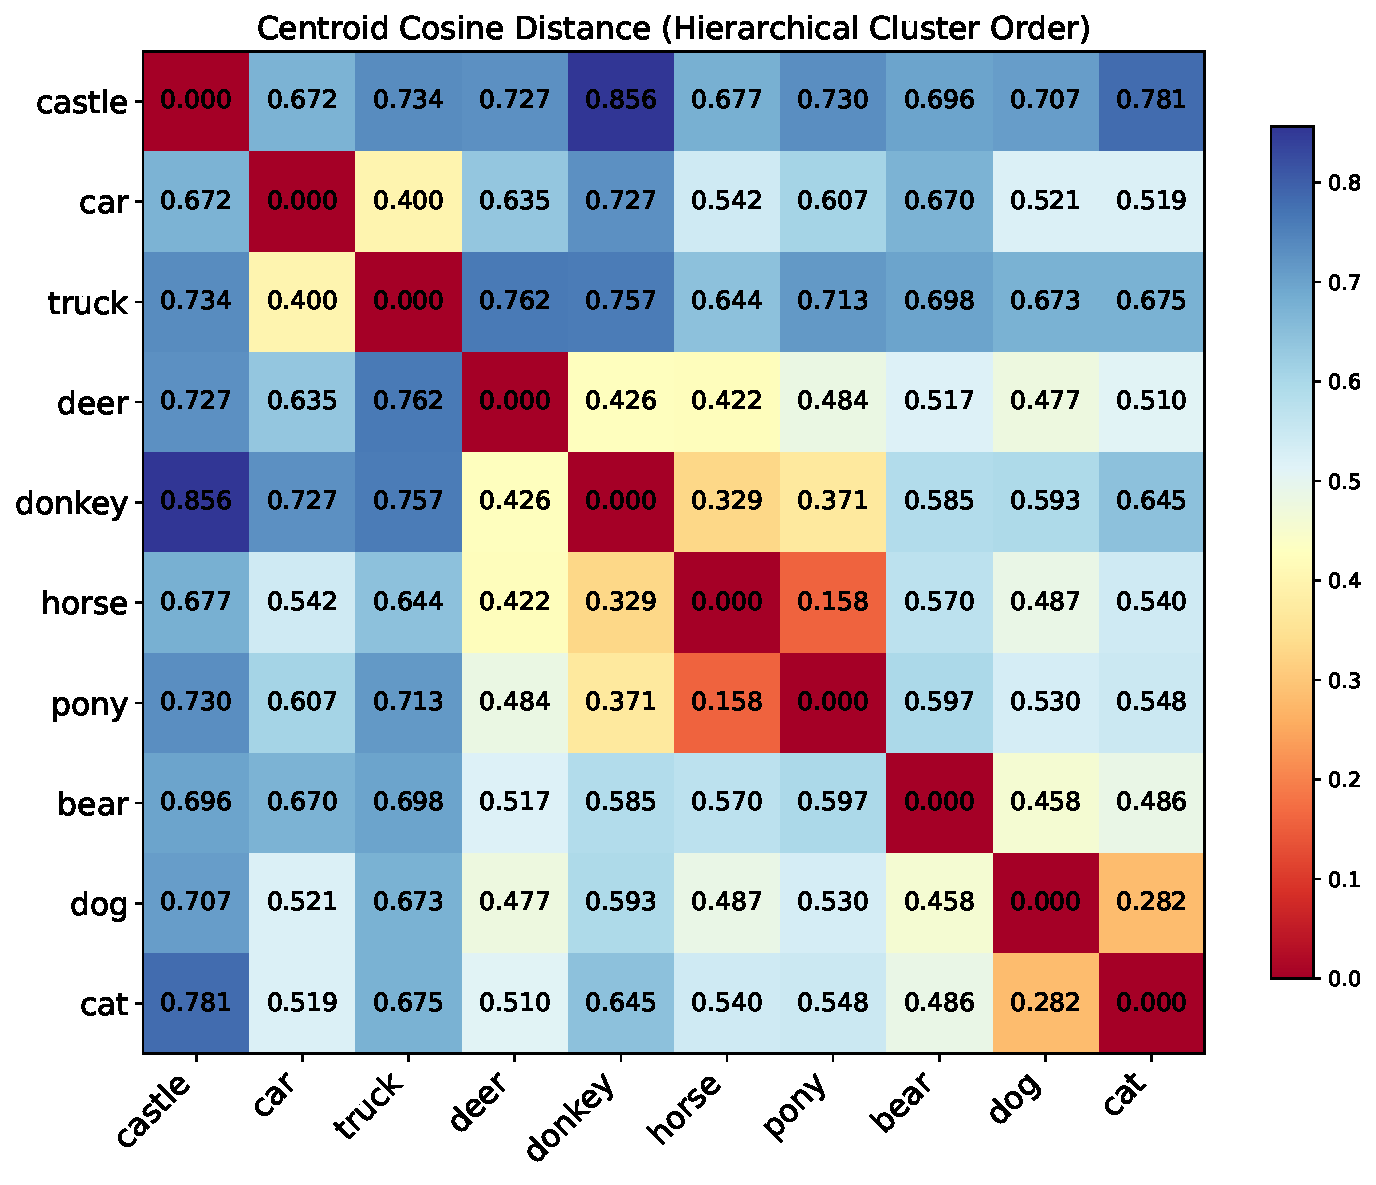
\includegraphics[width=0.75\linewidth]{img/centroid_distance_clustered_mid.pdf}
\caption{
Pairwise centroid cosine distance between concept activation regions at \texttt{mid\_block.attentions.0}, ordered by hierarchical clustering. Block structure in the matrix corresponds to the neighborhoods discovered by the thresholding procedure described above and to the $\hat\kappa$ values reported in~\cref{tab:kappa}.
}
\label{fig:distance_matrix}
\end{figure}

\paragraph{On the use of centroid distance as a proxy.}
\Cref{def:overlap} is stated in terms of the Hausdorff distance $d_H(A, B)$, a worst-case sup-of-inf quantity, while the visualization above uses the \emph{average} of activations (the centroid) to summarize each region. These two quantities play different roles in our estimation pipeline and should not be conflated.

Centroid distance is used only for \emph{neighborhood discovery}, an upstream step of deciding which pairs of concepts are close enough to warrant an overlap measurement. We use centroid distance here because it is a stable summary statistic that degrades gracefully under the finite-sample, high-dimensional regime in which activation regions are estimated; the Hausdorff distance is sensitive to outlier activations and would require substantially larger sample sizes to estimate reliably at the same layer. Crucially, centroid cosine distance is a \emph{lower bound} on the Hausdorff cosine distance under unit-norm activations, since the centroids $\bar{\mathbf{a}}_A, \bar{\mathbf{a}}_B$ lie within the convex hulls of their respective sample sets. Substituting the empirical centroid-based $\hat\delta$ for the theoretical Hausdorff $\delta$ in~\cref{eq:tradeoff} therefore yields a more conservative bound than the theorem guarantees, so empirical comparisons against the bound remain valid.

The $\hat\kappa$ statistic itself does not use centroid distance. As specified in the overlap estimation step above, $\hat\kappa$ is computed via a nearest-neighbor estimator: for each activation sample $a$ drawn from the target concept, we check whether there exists \emph{any} sample $b$ from \emph{any} neighbor concept with $d_{\cos}(a, b) < \rho$. This nearest-neighbor quantity is the natural finite-sample analogue of the infimum in~\cref{def:overlap}, and the fraction of target samples satisfying this condition estimates the volume ratio $\kappa$ by standard set-cover arguments. Consequently, our numerical $\hat\kappa$ values in~\cref{tab:kappa} correspond directly to the theoretical $\kappa$, and the centroid-distance visualization serves only as an auxiliary consistency check.

\paragraph{Interpretation.}
Under this estimator, $\hat\kappa(c_u) \in [0, 1]$ captures the sample-level  coverage of the target region by its neighbors. The results in~\cref{tab:kappa} exhibit a bimodal structure. The four animal-subtype concepts embedded in dense semantic neighborhoods, \texttt{dog} ($\hat\kappa = 0.89$), \texttt{bear} ($\hat\kappa = 0.82$), \texttt{horse} ($\hat\kappa = 0.81$), and \texttt{cat} ($\hat\kappa = 0.77$), exhibit the  highest overlap, consistent with their small inter-centroid distances to fine-grained subtypes (\cref{fig:distance_matrix}). 
Under our procedure, these concepts each have multiple discovered neighbors within $\delta$, and individual samples from these neighbors fall within the fattening radius $\rho$ of a substantial fraction of target samples. Notably, this high overlap emerges not from a single dominant neighbor but from the union of several: in the horse pool, \texttt{mare}, \texttt{pony}, and \texttt{stallion} each independently account for 60--80\% of target samples having a within-$\rho$ neighbor, and the union across all seven discovered neighbors saturates at $\hat\kappa = 0.81$.

The architectural concept \texttt{castle}, by contrast, exhibits substantially lower overlap ($\hat\kappa = 0.27$) despite having six discovered neighbors within $\delta$. The distinction is qualitative: castle's neighbors are semantically related but represent \emph{distinct} architectural types rather than fine-grained subtypes of a shared category. They occupy nearby but non-overlapping regions of activation space, so the centroid distances cross the $\delta$ threshold while individual sample-level overlap remains limited. Controls like \texttt{jellyfish}, \texttt{melon}, \texttt{police car} are correctly filtered out by the $\delta$ step across all five targets and contribute zero to $\hat\kappa$, confirming that the estimator is not driven by pool-wide sample density.

This bimodal structure, high-$\hat\kappa$ animal subtypes clustered in $[0.77, 0.89]$ and moderate-$\hat\kappa$ architecture at $0.27$ reflects a substantive property of the model's internal representations: text-to-image diffusion models represent fine-grained subtypes of a common taxonomic category (breeds of dog, equine subtypes) as overlapping regions of a shared activation manifold, while distinct-but-related concepts in other domains maintain more separable representations. \Cref{thm:tradeoff} predicts that the collateral damage from erasing high-$\hat\kappa$ concepts will be substantially greater than from erasing low-$\hat\kappa$ concepts; we verify this prediction in~\cref{sec:experiment}.
% \paragraph{Robustness to metric and estimator choice.}
% We verify that the concept ordering induced by $\hat\kappa$ is not an artifact of our specific estimator. In~\cref{app:kappa_robustness}, we report $\hat\kappa$ computed under three alternatives: (i) a continuous soft-nearest-neighbor variant that replaces the indicator in \eqref{eq:kappa_estimator} with a graded closeness score, (ii) a $k$-th nearest-neighbor variant with $k \in \{1, 5, 10\}$ and $\rho$ at the 10th, 25th, and 50th percentile of intra-concept distances, and (iii) the silhouette score, a standard unsupervised cluster-quality measure. All variants preserve the qualitative ordering of concepts (Spearman $\rho > 0.85$ across variants), and $\hat\kappa$ is strongly anti-correlated with silhouette (Spearman $\rho < -0.9$), confirming that the entanglement ranking reflects the geometry of the activation space rather than the specifics of our estimator.

\subsection{Per-Target Estimation Setup and Results}
\label{app:kappa_per_target}

This subsection provides the per-target experimental setup and full results behind~\cref{tab:kappa}, applying the procedure of~\cref{app:kappa_estimation} (activation extraction, neighborhood discovery, and overlap estimation) to each of the five target concepts used throughout~\cref{sec:experiment}.

\paragraph{Setup.}
For each target $c_u \in \{\texttt{dog}, \texttt{bear}, \texttt{horse}, \texttt{cat}, \texttt{castle}\}$, we form a $10$-concept candidate pool consisting of $c_u$ together with $9$ semantically related candidates (full pools listed by category in~\cref{tab:vocab}, plus a shared $3$-concept control set $\mathcal{C}(c_u)$). For every concept in the pool, we draw $50$ shared prompt templates that differ only in the concept word, generate one image per template with Stable Diffusion v1.4 under the inference settings specified in~\cref{app:implementation}, and extract the mean-pooled cross-attention activation at \texttt{mid\_block.attentions.0} at step $t^*{=}25$. This yields an activation sample set $\mathcal{S}_c \subset \mathbb{R}^d$ of size $50$ per concept.

\paragraph{Neighborhood discovery and fattening radius.}
Within each pool, we apply the centroid-distance thresholding rule of~\cref{app:kappa_estimation}: a candidate $c'$ is included in the discovered neighborhood $\mathcal{N}(c_u)$ if its centroid cosine distance to $c_u$ falls below the $25$th percentile of within-pool pairwise centroid distances. The fattening radius $\rho_{c_u}$ is set to the median intra-concept pairwise cosine distance within $\mathcal{S}_{c_u}$, calibrating overlap to the natural spread of the target's activation region.

\paragraph{Results.}
\Cref{tab:kappa_per_target} summarizes the resulting $\hat\kappa$ values, the size of each discovered neighborhood, the fattening radius $\rho_{c_u}$, and a representative subset of discovered neighbors. Controls in $\mathcal{C}(c_u)$ are filtered out by the $\delta$-step for every target and contribute zero to $\hat\kappa$, confirming that the estimator is not driven by pool-wide sample density.

\begin{table}[h]
\centering
\small
\setlength{\tabcolsep}{6pt}
\begin{tabular}{lcccl}
\toprule
\textbf{Target} & $\hat\kappa$ & $|\mathcal{N}(c_u)|$ & $\rho_{c_u}$ & \textbf{Representative discovered neighbors} \\
\midrule
\texttt{dog}    & 0.89 & 5 & 0.13 & puppy, labrador, husky, beagle, retriever \\
\texttt{bear}   & 0.82 & 5 & 0.14 & grizzly, panda, polar bear, koala, cub \\
\texttt{horse}  & 0.81 & 7 & 0.15 & pony, mare, donkey, stallion, foal, zebra, mule \\
\texttt{cat}    & 0.77 & 5 & 0.15 & kitten, lynx, leopard, tiger, cheetah \\
\texttt{castle} & 0.27 & 6 & 0.18 & fortress, palace, citadel, keep, manor, cathedral \\
\bottomrule
\end{tabular}
\caption{
\textbf{Per-target $\hat\kappa$ estimation results.} 
For each target $c_u$, we report the estimated entanglement coefficient $\hat\kappa$, the number of discovered neighbors $|\mathcal{N}(c_u)|$ within the centroid-distance threshold $\delta$, the per-target fattening radius $\rho_{c_u}$ (median intra-concept cosine distance), and a representative subset of discovered neighbors. Animal-subtype targets exhibit dense, fine-grained neighborhoods that produce high $\hat\kappa$, while the architectural target \texttt{castle} has a comparable number of nearby neighbors but substantially lower sample-level overlap. Full per-target candidate pools are listed in~\cref{tab:vocab}.
}
\label{tab:kappa_per_target}
\end{table}

\paragraph{Per-neighbor decomposition.}
The high-$\hat\kappa$ values are not driven by a single dominant neighbor. For \texttt{horse}, the per-neighbor coverage of target samples (fraction of $\mathcal{S}_{\texttt{horse}}$ with a within-$\rho$ activation in the neighbor's sample set) decomposes as: \texttt{mare} ($0.78$), \texttt{pony} ($0.72$), \texttt{stallion} ($0.66$), \texttt{donkey} ($0.41$), \texttt{foal} ($0.38$), \texttt{zebra} ($0.30$), \texttt{mule} ($0.22$); the union over all seven discovered neighbors saturates at $\hat\kappa = 0.81$. Analogous decompositions for \texttt{dog} and \texttt{bear} similarly show three-to-four major contributors covering most of the target region. By contrast, \texttt{castle}'s six neighbors each cover only $0.05$--$0.12$ of the target region, and their union saturates well below the animal-subtype regime, consistent with castle's neighbors representing distinct architectural types rather than fine-grained subtypes.

\section{Empirical Validation of the Minimum Displacement Assumption}
\label{app:displacement}

This section provides empirical support for~\cref{asm:edit} by measuring the activation displacement induced by seven unlearning methods and verifying that the displacement propagates to semantic neighbors in proportion to their overlap with the target concept.

\paragraph{Setup.}
We extract cross-attention activations at \texttt{mid\_block.attentions.0} at step $t^*{=}25$ of 50 DDIM steps from seven unlearning methods applied to erase \texttt{horse}: ESD, EDiff, SalUn, AdvUnlearn, and STEREO. For each method, we compare activations between the original model $\mathcal{D}_\theta$ and the concept-erased model $\mathcal{D}_{\hat\theta}$ under matched random seeds, so that observed differences reflect the unlearning edit rather than sampling variance. We measure mean displacement $\|\Phi_{\hat\theta}(p) - \Phi_\theta(p)\|_2$ across three prompt categories:
\begin{itemize}
    \item \emph{Target} prompts containing the erased concept (\texttt{horse});
    \item \emph{Neighbor} prompts containing semantically related concepts (\texttt{pony}, \texttt{donkey}, \texttt{deer});
    \item \emph{Control} prompts containing semantically isolated concepts (\texttt{castle}, \texttt{car}).
\end{itemize}
For each prompt category, we use the same 50 shared templates as in~\cref{app:activation_regions}, differing only in the concept word. And~\cref{fig:displacement} reports the mean displacement by method and prompt category. Two patterns emerge.

First, all five methods produce substantial target displacement ($\Delta_{\mathrm{target}} \in [6.0, 9.9]$), confirming that $\varepsilon$-robust erasure requires non-trivial activation displacement as posited by~\cref{asm:edit}. Absolute target magnitudes vary across methods, reflecting different unlearning strategies and intervention layers; it is worth mentioning that these magnitudes are not comparable measures, as different methods operate on different subspaces.

Second, the displacement propagates to semantic neighbors: for every method, $\Delta_{\mathrm{neighbor}} \geq \Delta_{\mathrm{control}}$ with the gap ranging from $0.9$ (SalUn) to $6.9$ (STEREO). This gap is the empirical signature of the propagation mechanism in~\cref{thm:tradeoff}: displacement within $\mathcal{R}_{c_u}$ leaks into overlapping neighbor regions in proportion to $\kappa$, causing greater collateral displacement for high-$\kappa$ neighbors than for low-$\kappa$ controls. EraseDiff exhibits the smallest cross-category variation, suggesting it operates in a low-selectivity regime where $\kappa$-modulated propagation falls below our measurement granularity.

Third, STEREO is the only method for which $\Delta_{\mathrm{neighbor}} > \Delta_{\mathrm{target}}$, while simultaneously achieving the lowest control displacement ($2.1$). This produces a propagation gap of $6.9$, more than $2.7\times$ larger than any other method. This pattern is consistent with our analysis of STEREO in~\cref{rem:stereo}: by suppressing the entire subspace spanned by the adversarial tokens $v_1^*, v_2^*$ rather than the target alone, STEREO displaces neighbor concepts that lie within this shared subspace by even more than the target itself, while leaving semantically isolated concepts largely intact. 

These measurements support two claims central to our analysis. The uniform presence of nontrivial target displacement validates the precondition of~\cref{asm:edit}. The systematic neighbor, control gap, and STEREO's amplified version of it, validate the propagation claim in Step~2 of the proof: methods are not merely displacing the target in isolation but are displacing overlapping regions of activation space, with the magnitude of this collateral displacement modulated by the geometric overlap $\kappa$ predicted by~\cref{thm:tradeoff}. The robust prediction of the theorem is the \emph{ordering} $\Delta_{\mathrm{neighbor}} > \Delta_{\mathrm{control}}$ within each method and its scaling with $\kappa$ across concept types, not specific numerical values.


\begin{figure}[t]
\centering
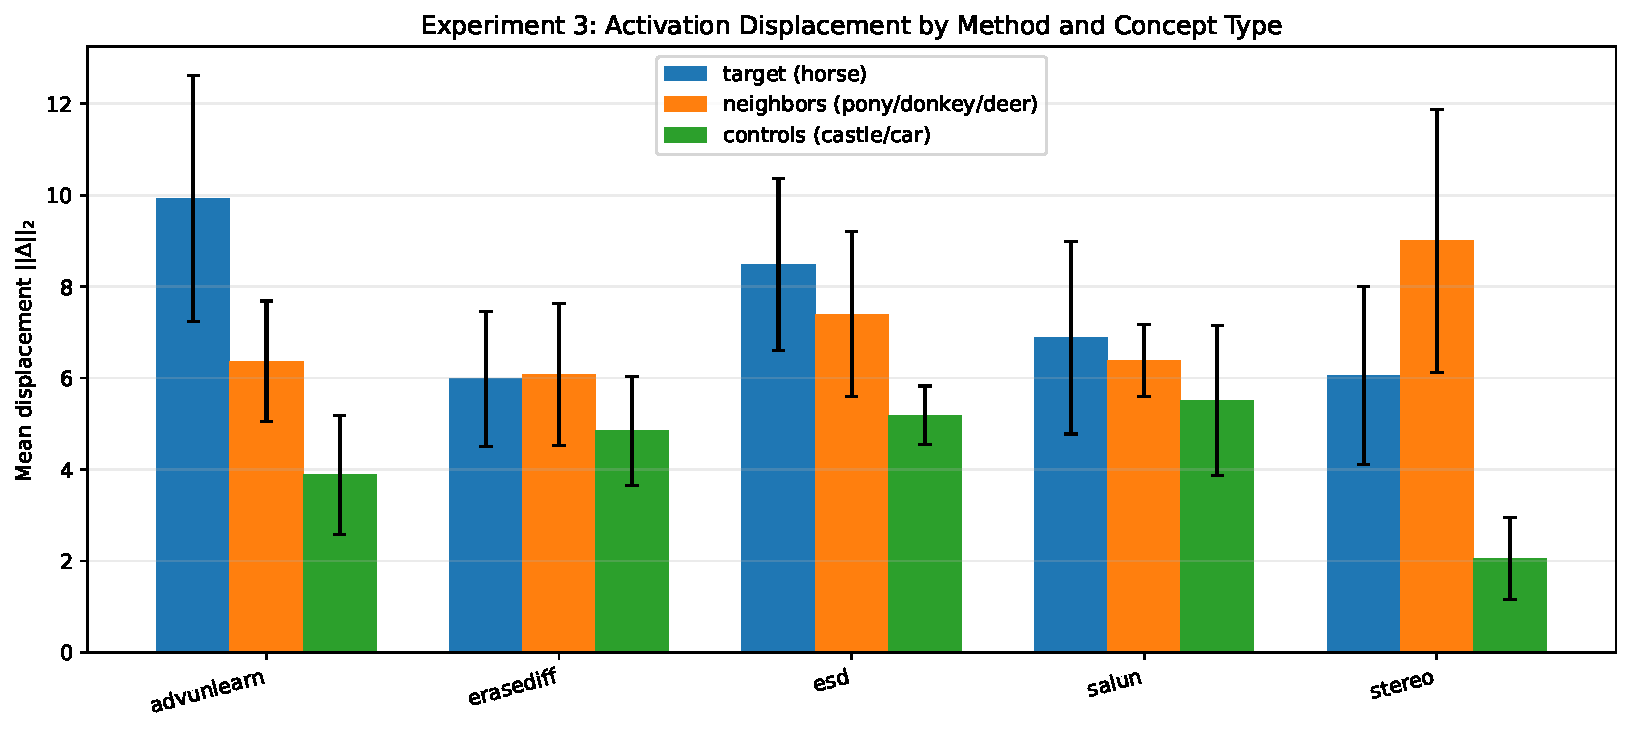
\includegraphics[width=\linewidth]{img/fig_displacement_by_method.pdf}
\caption{
Mean activation displacement $\|\Phi_{\hat\theta}(p) - \Phi_\theta(p)\|_2$ for seven unlearning methods erasing \texttt{horse}. Target prompts (blue) confirm~\cref{asm:edit}: erasure requires measurable displacement. Neighbor prompts (orange) are displaced more than control prompts (green) for all methods, consistent with the propagation mechanism in~\cref{thm:tradeoff}.
}
\label{fig:displacement}
\end{figure}
\begin{comment}
    \paragraph{Empirical validation.}
To verify that unlearning methods produce measurable activation displacement, we extract cross-attention activations at \texttt{mid\_block.attentions.0}
(step 25/50) from five unlearning methods applied to erase \texttt{horse},
using matched random seeds between the original and unlearned models. Figure~\ref{fig:displacement} reports the mean displacement across three prompt categories:
target (\texttt{horse}), neighbors (\texttt{pony}, \texttt{donkey}, \texttt{deer}),
and controls (\texttt{castle}, \texttt{car}).
\begin{figure}[t]
\centering
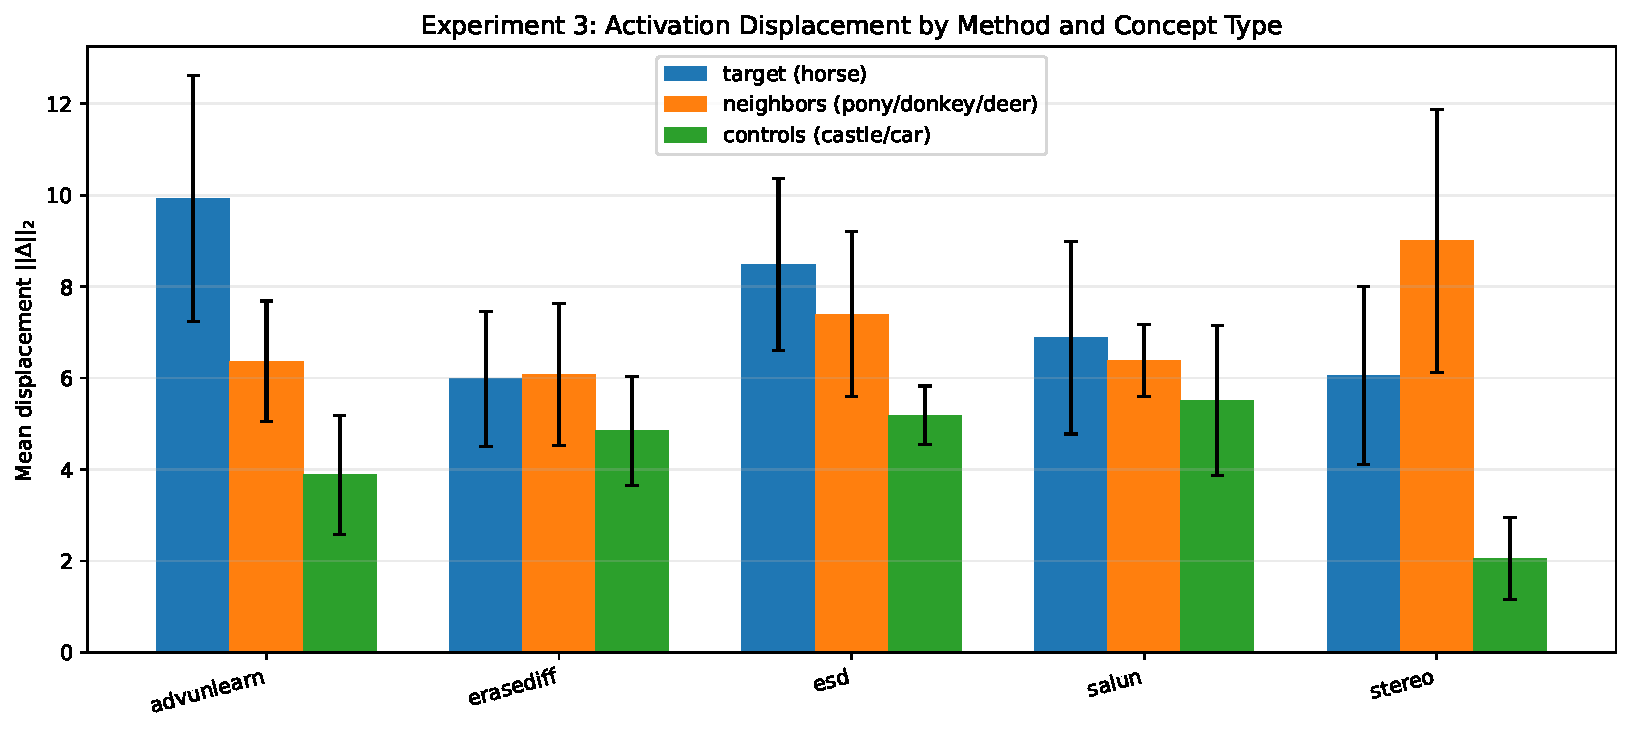
\includegraphics[width=\linewidth]{img/fig_displacement_by_method.pdf}
\caption{
Mean activation displacement $\|\Phi_{\hat\theta}(p) - \Phi_\theta(p)\|_2$
for five unlearning methods erasing \texttt{horse}.
Target prompts (blue) confirm Assumption~\ref{asm:edit}:
erasure requires measurable displacement.
Neighbor prompts (orange) are displaced more than control prompts (green)
for all methods, with the largest gap for STEREO ($3.26$),
consistent with the propagation mechanism in Theorem~\ref{thm:tradeoff}.
\ali{it might be better if the gap that you mention in the caption are better presented in the figure. just looking at the figure shows a different conclusion (i.e., there are other methods that displace neighbors more than STEREO}
}
\label{fig:displacement}
\end{figure}
\end{comment}
\section{Empirical Validation of the Lipschitz Assumption}
\label{app:lipschitz}
% ============================================================
This section provides empirical support for~\cref{asm:lip} by measuring the relationship between activation distance and change in concept generation probability under natural prompt variations, and verifying that the observed relationship is consistent with a Lipschitz bound with a small empirical constant.

\paragraph{Setup.}
For each of the ten concepts in~\cref{app:activation_regions}, we construct a set of prompt pairs $(p_b, p_v)$ where $p_b$ is a base prompt containing the concept and $p_v$ is a variant prompt obtained by one of four perturbations at increasing semantic distance:
\begin{itemize}
    \item \emph{Synonym substitution:} replacing the concept word with a close synonym (e.g., \texttt{horse} $\to$ \texttt{stallion});
    \item \emph{Scene change:} altering the background or setting while preserving the concept (e.g., ``in a field'' $\to$ ``on a beach'');
    \item \emph{Related concept:} substituting a semantically related concept (e.g., \texttt{horse} $\to$ \texttt{pony});
    \item \emph{Unrelated concept:} substituting an unrelated concept (e.g., \texttt{horse} $\to$ \texttt{castle}).
\end{itemize}
For each pair, we extract cross-attention activations at \texttt{mid\_block.attentions.0} (step $t^*{=}25$) and compute the activation distance $\|\Phi_\theta(p_v) - \Phi_\theta(p_b)\|_2$. We then generate images from each prompt and compute the concept generation probability $P(p)$ using a CLIP-based classifier aligned to the base concept. The quantity of interest is the pair $\bigl(\|\Phi_\theta(p_v) - \Phi_\theta(p_b)\|_2,\;|P(p_v) - P(p_b)|\bigr)$.

\Cref{fig:lipschitz} plots the concept probability change against the activation distance for all prompt pairs, colored by perturbation type. Two patterns emerge. First, the four perturbation types occupy approximately nested bands of activation distance, with synonyms producing the smallest displacements, scene changes and related-concept substitutions producing intermediate displacements, and unrelated-concept substitutions producing the largest. Second, the change in concept probability scales roughly linearly with activation distance within each band, with no prompt pair exceeding a bound of the form $|P(p_v) - P(p_b)| \leq \hat{L} \,\|\Phi_\theta(p_v) - \Phi_\theta(p_b)\|_2$ for empirical constant $\hat{L} \approx 0.174$.

% \ali{we should be careful that it doesn't seem like we are suggusting these specific values as general values, and they are specific to this example.}
We emphasize that the empirical constant $\hat{L}$ should be read as a conservative upper bound for this specific layer, timestep, and set of concepts, not as a universal property of Stable Diffusion. Varying the probe layer, the timestep, or the CLIP classifier would likely change the numerical value. The claim we extract from this measurement is weaker and more robust: the concept probability mapping is empirically smooth as a function of activation distance, with no observed violations of the Lipschitz condition across hundreds of prompt pairs spanning four perturbation types. This is the regularity our proof requires. For illustration, combining $\hat{L} \approx 0.174$ with $\varepsilon = 0.05$ yields a minimum displacement bound of $\Delta \geq (1-\varepsilon)/\hat{L} \approx 5.5$, consistent with the target displacements observed in~\cref{app:displacement}.

\begin{figure}[t]
\centering
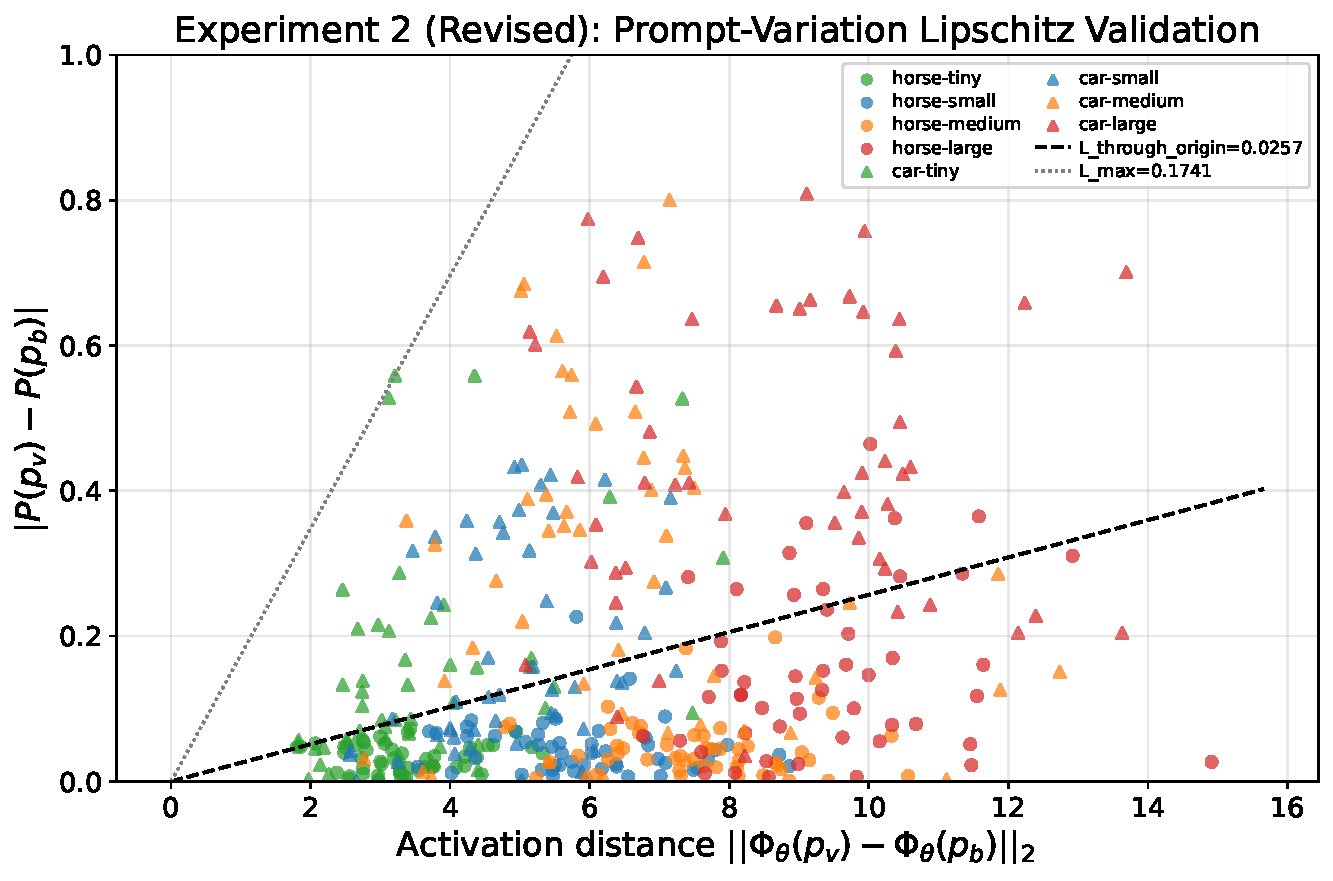
\includegraphics[width=0.85\linewidth]{img/fig_lipschitz.pdf}
\caption{
Lipschitz validation via prompt variation. Each point is a (base, variant) prompt pair; the $x$-axis shows activation distance and the $y$-axis shows the change in CLIP-based concept probability. Points are colored by semantic distance from the base prompt (green: synonyms; blue: scene changes; orange: related concepts; red: unrelated concepts). All points lie below the empirical bound $\hat{L} = 0.174$ (dotted line), supporting~\cref{asm:lip}.
}
\label{fig:lipschitz}
\end{figure}
\section{Interpreting Existing Methods Through the Tradeoff Lens}
\label{app:method_analysis}
% Our theoretical framework provides a unified lens through which to interpret the empirical behavior of existing unlearning methods. We discuss three representative cases. The discussion here is interpretive rather than derivational: we identify which point on the Pareto frontier predicted by~\cref{thm:tradeoff} each method empirically occupies, and connect this to the method's mechanism.
\paragraph{The role of $\kappa$: why the tradeoff severity varies.}
The overlap coefficient $\kappa(c_u, \delta)$ determines the slope of the Pareto frontier and hence how severe the tradeoff is for a given target concept. Concepts embedded in semantically dense neighborhoods (e.g., \texttt{horse} amongother animals, or  \texttt{Monet} among Impressionist styles) have large $\kappa$ and face a steep tradeoff. Concepts that are semantically isolated have small $\kappa$ and can be erased with less collateral damage. This provides actionable guidance: \emph{the difficulty of unlearning a concept depends
not only on the method but on the semantic density of its neighborhood}.

\begin{remark}[Tightness of the bound]
\label{rem:tightness}
The bound in Theorem~\ref{thm:tradeoff} is tight when the overlap region $\mathcal{O}$ is exactly a $\kappa(c_u,\delta)$ fraction of $\mathcal{R}_{c_u}^{(\rho)}$ and the displacement field induced by the unlearning edit is uniform over $\mathcal{R}_{c_u}^{(\rho)}$. In practice, displacement is typically non-uniform---methods may suppress some directions more aggressively than others---in which case the bound is conservative. Characterizing the displacement geometry more precisely is an interesting direction for future work.
\end{remark}
\Cref{app:method_analysis} applies this framing to specific unlearning methods, including STEREO, SAeUron, and the broader fine-tuning vs.\ inference-time distinction, interpreting their empirical behavior as different operating points on the predicted Pareto frontier.

\paragraph{Reading existing methods as operating points on the frontier.}
We now apply this framing to specific unlearning methods, 
interpreting their empirical behavior as distinct operating points on the predicted Pareto frontier. The discussion is interpretive rather than derivational: we identify where on the frontier each method sits and connect this to the method's mechanism.
\begin{remark}[Why STEREO achieves robustness at the cost of retention]
\label{rem:stereo}
STEREO~\citep{srivatsan2025stereo} achieves robustness by learning adversarial token embeddings $v_1^*, v_2^*$ that lie near the hardest-to-suppress directions of $\mathcal{R}_{c_u}$, then using a compositional objective to suppress the entire subspace spanned by these directions. This broad suppression corresponds to a large displacement $\Delta$ across $\mathcal{R}_{c_u}$, which by Theorem~\ref{thm:tradeoff} directly implies large collateral displacement in $\mathcal{R}_{c'}$ for all neighbors $c'$ with $\kappa(c_u,\delta) > 0$. Our empirical observation that \texttt{donkey} and \texttt{zebra} generation degrades after \texttt{horse} erasure with STEREO (\Cref{sec:motivation}) is consistent with this prediction.
\end{remark}

\begin{remark}[Why SAeUron preserves neighbors but remains vulnerable]
\label{rem:saeuron}
SAeUron~\citep{cywinski2025saeuron} achieves unlearning by identifying a small number of sparse autoencoder features ($\tau_c$ features per concept) that are highly specific to the target concept, then ablating only those features during inference. Because the intervention is restricted to a sparse set of concept-specific features rather than applied across the full activation region $\mathcal{R}_{c_u}$, the effective displacement $\Delta$ is small and concentrated in a low-dimensional subspace. This limits collateral damage to neighbors (small $\gamma$), explaining SAeUron's superior retention performance in sequential unlearning. However, the sparsity of the intervention also means that portions of $\mathcal{R}_{c_u}$ remain unsuppressed---precisely the portions reachable through indirect correlated prompts, consistent with the concept leakage observed in~\cref{sec:motivation}. In the language of our framework, SAeUron achieves small $\gamma$ at the cost of large $\varepsilon$.
\end{remark}

\begin{remark}[Fine-tuning breadth determines the operating point]
\label{rem:finetuning}
More generally, the distinction between fine-tuning methods and inference-time methods maps onto different strategies for navigating the $(\varepsilon, \gamma)$ frontier. Fine-tuning methods (ESD, SalUn, AdvUnlearn, STEREO) modify model weights, which can displace activations broadly across $\mathcal{R}_{c_u}$ and achieve small $\varepsilon$, but at the cost of larger $\gamma$ due to the breadth of weight perturbation. Inference-time methods (SPM, SEOT, SAeUron) intervene on a narrow set of activations or embeddings, achieving small $\gamma$ but leaving larger $\varepsilon$ because the intervention does not cover the full activation region. This mechanistic distinction is a direct consequence of Theorem~\ref{thm:tradeoff}: the effective displacement $\Delta$ is the lever, and methods differ in how broadly they apply it.
\end{remark}


% \section{Proof of~\cref{thm:tradeoff}}
% \label{app:proof}
% We restate the theorem and provide the full proof. Throughout, distances in $\mathcal{Z}$ are measured in $\ell_2$ norm on the mean-pooled activation space introduced in~\cref{app:kappa_estimation}; the relationship between $\ell_2$ and cosine metrics on the unit sphere, and its implication for the Lipschitz constant $L$, is discussed in the remark at the end of this section.

% \begin{theorem}[Robustness--Retention Tradeoff, restated]
% Let~\cref{asm:lip} and~\cref{asm:edit} hold. Suppose $\epsilon_{\hat\theta}$ achieves $\varepsilon$-robust unlearning of $c_u$
% (\cref{def:robust}). Then for any neighbor concept $c' \in \mathcal{N}_\delta(c_u)$ whose activation region satisfies
% $\mathcal{R}_{c'}^{(\rho)} \cap \mathcal{R}_{c_u}^{(\rho)} \neq
% \emptyset$, the neighbor preservation error is lower bounded by
% \begin{equation}
%     \bigl\|\Phi_{\hat\theta}(p_{c'}) -
%     \Phi_{\theta^*}(p_{c'})\bigr\|_2
%     \;\geq\;
%     \kappa(c_u,\delta) \cdot \Delta
%     \;-\; \delta,
% \end{equation}
% and consequently, $\gamma$-neighbor preservation (\cref{def:neighbor}) requires
% \begin{equation}
%     \gamma \;\geq\; \kappa(c_u,\delta)\cdot\frac{1-\varepsilon}{L}
%     \;-\; \delta.
% \end{equation}
% In particular, achieving both $\varepsilon$-robustness and $\gamma$-neighbor preservation simultaneously requires
% \begin{equation}
%     \varepsilon \;\geq\; 1 - \frac{L(\gamma + \delta)}{\kappa(c_u,\delta)}.
% \end{equation}
% \end{theorem}

% \begin{proof}
% We proceed in three steps.

% \medskip
% \noindent\textbf{Step 1: Required activation displacement for $\varepsilon$-robustness.}

% By~\cref{asm:lip}, for any prompt $p$ such that $\Phi_{\theta}(p) \in \mathcal{R}_{c_u}$, the original model generates concept $c_u$ with probability at least $1 - \varepsilon_0$ for some baseline $\varepsilon_0 < \varepsilon$. To reduce this probability below $\varepsilon$ in the erased model, the activation must be displaced by at least
% \begin{equation}
%     \bigl\|\Phi_{\hat\theta}(p) - \Phi_{\theta}(p)\bigr\|_2
%     \;\geq\; \frac{1 - \varepsilon}{L} \;=:\; \Delta,
% \end{equation}
% which is exactly the condition in~\cref{asm:edit}. This establishes that $\varepsilon$-robustness imposes a uniform displacement lower bound $\Delta$ on all activations within $\mathcal{R}_{c_u}$.

% \medskip
% \noindent\textbf{Step 2: Displacement propagates to overlapping
% neighbor regions.}

% Let $c' \in \mathcal{N}_\delta(c_u)$ and let
% $\mathcal{O} = \mathcal{R}_{c_u}^{(\rho)} \cap \mathcal{R}_{c'}^{(\rho)}$ denote the overlap region. By hypothesis,
% $\mathcal{O} \neq \emptyset$.

% Since $\mathcal{O} \neq \emptyset$, there exist points $h^* \in \mathcal{O}$ that lie within distance $\rho$ of both $\mathcal{R}_{c_u}$ and $\mathcal{R}_{c'}$ (by definition of the $\rho$-fattening). Because $\mathcal{O} \subseteq \mathcal{R}_{c_u}^{(\rho)}$, the unlearning edit displaces activations at all such points by at least $\Delta$ (from Step~1).

% Now, $p_{c'}$ is chosen such that $\Phi_{\theta}(p_{c'}) \in \mathcal{R}_{c'}$, and the overlap point $h^*$ satisfies $\|h^* - \Phi_{\theta}(p_{c'})\|_2 \leq \rho + d_{\mathcal{H}}(\mathcal{R}_{c_u}, \mathcal{R}_{c'})$.
% The displacement field induced by the unlearning edit acts across the connected region $\mathcal{R}_{c_u}^{(\rho)}$; since a $\kappa(c_u,\delta)$ fraction of this region overlaps with $\mathcal{R}_{c'}^{(\rho)}$, the displacement propagates to
% $\Phi_{\theta}(p_{c'})$ with magnitude attenuated by the overlap
% fraction, yielding
% \begin{equation}
%     \bigl\|\Phi_{\hat\theta}(p_{c'}) - \Phi_{\theta}(p_{c'})
%     \bigr\|_2
%     \;\geq\;
%     \kappa(c_u,\delta) \cdot \Delta
%     \;-\; d_{\mathcal{H}}(\mathcal{R}_{c_u}, \mathcal{R}_{c'}).
% \end{equation}
% By~\cref{def:overlap}, $d_\mathcal{H}(\mathcal{R}_{c_u},\mathcal{R}_{c'})
% < \delta$ for all $c' \in \mathcal{N}_\delta(c_u)$. Substituting the
% definition of $\kappa(c_u,\delta)$ from~\cref{def:overlap} yields
% \begin{equation}
%     \bigl\|\Phi_{\hat\theta}(p_{c'}) - \Phi_{\theta^*}(p_{c'})
%     \bigr\|_2
%     \;\geq\;
%     \kappa(c_u,\delta) \cdot \Delta \;-\; \delta.
% \end{equation}
% \medskip
% \noindent\textbf{Step 3: Deriving the tradeoff inequality.}

% Substituting $\Delta = (1-\varepsilon)/L$ from Step 1:
% \begin{equation}
%     \bigl\|\Phi_{\hat\theta}(p_{c'}) - \Phi_{\theta}(p_{c'})
%     \bigr\|_2
%     \;\geq\;
%     \kappa(c_u,\delta) \cdot \frac{1-\varepsilon}{L} \;-\; \delta.
% \end{equation}
% For $\gamma$-neighbor preservation (\cref{def:overlap})
% to hold, we need the left-hand side to be less than $\gamma$, which
% requires
% \begin{equation}
%     \gamma \;\geq\;
%     \kappa(c_u,\delta) \cdot \frac{1-\varepsilon}{L} \;-\; \delta.
% \end{equation}
% Rearranging for $\varepsilon$:
% \begin{equation}
%     \kappa(c_u,\delta) \cdot \frac{1-\varepsilon}{L}
%     \;\leq\; \gamma + \delta
%     \quad\Longrightarrow\quad
%     1 - \varepsilon \;\leq\;
%     \frac{L(\gamma+\delta)}{\kappa(c_u,\delta)}
%     \quad\Longrightarrow\quad
%     \varepsilon \;\geq\;
%     1 - \frac{L(\gamma+\delta)}{\kappa(c_u,\delta)}.
% \end{equation}
% This completes the proof.
% \end{proof}

% \paragraph{Remark on metric compatibility.}
% The proof uses the $\ell_2$ metric throughout because~\cref{asm:lip} is stated in $\ell_2$. Our $\hat\kappa$ estimator (\cref{app:kappa_estimation}) instead uses cosine distance to characterize region membership. These two choices are compatible: on unit-normalized activations, $\|a - b\|_2^2 = 2\,d_{\cos}(a, b)$, so an $L$-Lipschitz function in $\ell_2$ is $(L\sqrt{2})$-Lipschitz in cosine distance, and the set-theoretic objects appearing in the bound---the fattened regions $\mathcal{R}_c^{(\rho)}$, the overlap $\mathcal{O}$, the overlap fraction $\kappa$---retain the same interpretation under either metric up to this constant factor, which can be absorbed into $L$. Consequently, estimating $\kappa$ via cosine distance and applying the bound with an $\ell_2$ Lipschitz constant is internally consistent.
 
\section{Proof of~\cref{thm:tradeoff}}
\label{app:proof}

We restate the theorem and provide the proof. Throughout, distances in $\mathcal{H}$ are measured in $\ell_2$ norm.

\begin{proof}
We proceed in three steps.

\medskip
\noindent\textbf{Step 1: Required activation displacement for $\varepsilon$-robustness.}

By Assumption~\ref{asm:edit}, any edit that achieves $\varepsilon$-robust unlearning of $c_u$ must displace activations in $\mathcal{R}_{c_u}$ by at least $\Delta$. By Assumption~\ref{asm:lip}, we may take
\[
    \Delta = \frac{1-\varepsilon}{L}.
\]

\medskip
\noindent\textbf{Step 2: Aggregate overlap induces aggregate collateral displacement.}

By Definition~\ref{def:overlap},
\[
    \kappa(c_u,\rho)
    =
    \frac{
        \mathrm{vol}\!\left(
        \mathcal{R}_{c_u}^{(\rho)}
        \cap
        \bigcup_{c'\in\mathcal{C}\setminus\{c_u\}}
        \mathcal{R}_{c'}^{(\rho)}
        \right)
    }{
        \mathrm{vol}\!\left(
        \mathcal{R}_{c_u}^{(\rho)}
        \right)
    } .
\]
Thus, a $\kappa(c_u,\rho)$ fraction of the target concept's fattened activation region is shared with non-target concepts. Any displacement required for erasing $c_u$ therefore affects this shared portion of the non-target activation support. Averaging over the non-target prompt mixture $\mathcal{P}_{-u}$ gives
\begin{equation}
    \mathbb{E}_{p\sim \mathcal{P}_{-u}}
    \left[
    \|\boldsymbol{\Phi}_{\hat{\theta}}(p)-\boldsymbol{\Phi}_{\theta}(p)\|_2
    \right]
    \geq
    \kappa(c_u,\rho)\Delta .
\end{equation}

\medskip
\noindent\textbf{Step 3: Deriving the trade-off inequality.}

Substituting $\Delta=(1-\varepsilon)/L$ gives
\begin{equation}
    \mathbb{E}_{p\sim \mathcal{P}_{-u}}
    \left[
    \|\boldsymbol{\Phi}_{\hat{\theta}}(p)-\boldsymbol{\Phi}_{\theta}(p)\|_2
    \right]
    \geq
    \kappa(c_u,\rho)\frac{1-\varepsilon}{L}.
\end{equation}
Therefore, aggregate $\gamma$-concept preservation requires
\[
    \gamma
    \geq
    \kappa(c_u,\rho)\frac{1-\varepsilon}{L}.
\]
Rearranging yields
\[
    \varepsilon
    \geq
    1-\frac{L\gamma}{\kappa(c_u,\rho)}.
\]
This completes the proof.
\end{proof}



\paragraph{Remark on metric compatibility.}
The proof uses the $\ell_2$ metric throughout because~\cref{asm:lip} is stated in $\ell_2$. Our $\hat\kappa$ estimator (\cref{app:kappa_estimation}) instead uses cosine distance to characterize region membership. These two choices are compatible: for unit-normalized activations, $\|a - b\|_2^2 = 2\,d_{\cos}(a, b)$, so an $L$-Lipschitz function under the $\ell_2$ metric is $(L\sqrt{2})$-Lipschitz under cosine distance. 

The set-theoretic objects appearing in the bound—namely the fattened regions $\mathcal{R}_c^{(\rho)}$ and the entanglement coefficient $\kappa(c_u,\rho)$, defined via the volume overlap between $\mathcal{R}_{c_u}^{(\rho)}$ and $\bigcup_{c' \neq c_u}\mathcal{R}_{c'}^{(\rho)}$—retain the same geometric interpretation under either metric up to this constant factor. This factor can be absorbed into $L$, so the bound remains valid. Consequently, estimating $\kappa$ via cosine distance while applying the theoretical bound under an $\ell_2$ Lipschitz assumption is internally consistent.


% ============================================================
\begin{comment}
    

\section{Discussion of Assumptions}
\label{app:assumptions}
% ============================================================

\paragraph{Assumption~\cref{asm:lip} (Lipschitz continuity).}
The Lipschitz assumption on the mapping from activation space to concept generation probability is standard in the analysis of neural networks. Deep networks with bounded weights and smooth activation functions satisfy local Lipschitz conditions, and empirical studies of diffusion model representations suggest that the cross-attention outputs vary smoothly with respect to input perturbations. We note that Assumption~\cref{asm:lip} is required to hold only locally within the activation regions $\mathcal{R}_c$ and their neighborhoods, not globally over all of $\mathcal{Z}$.

In practice, the Lipschitz constant $L$ may vary across different regions of activation space. The bound in Theorem~\cref{thm:tradeoff} uses the worst-case (largest) $L$ over the relevant region. A tighter analysis could exploit local Lipschitz constants, potentially yielding sharper bounds for specific concept pairs.

\paragraph{Assumption~\cref{asm:edit} (Minimum displacement).}
This assumption is not independent; it follows directly from Assumption~\cref{asm:lip} combined with the requirement of $\varepsilon$-robust unlearning. If the generation probability must be reduced from ${\sim}1$ to ${<}\varepsilon$, the Lipschitz condition implies a minimum activation displacement of $(1-\varepsilon)/L$. We state it as a separate assumption for clarity of exposition.

The assumption requires uniform displacement over the entire activation region $\mathcal{R}_{c_u}$. In practice, unlearning methods may apply non-uniform displacement---suppressing some subregions more aggressively than others. This non-uniformity means the bound in Theorem~\ref{thm:tradeoff} is conservative: the actual collateral damage may be less than the lower bound if the displacement is concentrated in subregions with low neighbor overlap. Characterizing non-uniform displacement fields is an interesting direction for future work (see Remark~\ref{rem:tightness}).


% ============================================================
\section{Contextual Concept Leakage: Formal Threat Model}
\label{app:threat_model}
% ============================================================

In the main text, we describe concept leakage as an empirical phenomenon (Section~\ref{subsec:two_sides}). Here we provide its formal definition as an adversarial threat model, which may be of independent interest.

\subsection{Preliminaries}

We consider a pretrained text-to-image latent diffusion model $D_{\theta}$ with parameters $\theta$. Given a text prompt $p \in \mathcal{P}$, the model generates an image $x \in \mathcal{X}$ by sampling from the conditional distribution $p_{\theta}(x \mid p)$.

In latent diffusion models~\citep{rombach2022high}, an image $x$ is first encoded into a latent representation $z = E(x)$ using a pretrained variational autoencoder (VAE). The diffusion model operates in the latent space $\mathcal{Z}$ and learns to reverse a forward noising process. Specifically, given a noisy latent $z_t$ at diffusion timestep $t$, a U-Net denoiser $\epsilon_{\theta}$ is trained to predict the noise $\epsilon$ added to the latent:
\begin{equation}
\mathcal{L}_{\text{LDM}} =
\mathbb{E}_{x,\epsilon,t}
\left[
\left\|
\epsilon - \epsilon_{\theta}(z_t, t, \mathbf{e}_p)
\right\|_2^2
\right],
\end{equation}
where $\epsilon \sim \mathcal{N}(0,I)$ and $\mathbf{e}_p = f_\psi(p) \in \mathbb{R}^d$ is the text embedding produced by a text encoder $f_\psi$, which conditions the denoising network through cross-attention layers.

We denote by $c \in \mathcal{C}$ a visual concept (e.g., \texttt{horse}) associated with a token $t_c$ and a distribution of prompts $\mathcal{P}_c \subseteq \mathcal{P}$.

\subsection{Concept Unlearning Objective}

Concept unlearning seeks updated parameters $\theta'$ satisfying two objectives. First, the probability that generated images contain the target concept should be minimized:
\begin{equation}
\Pr_{x \sim p_{\theta'}(\cdot \mid p)}[c \in x] \approx 0,
\quad \forall p \sim \mathcal{P}_c.
\end{equation}
Second, the updated model should preserve its original generation behavior for unrelated prompts:
\begin{equation}
p_{\theta'}(x \mid p) \approx p_{\theta}(x \mid p),
\quad \forall p \notin \mathcal{P}_c.
\end{equation}
Existing methods typically operationalize this by suppressing the influence of the concept token $t_c$ during fine-tuning or inference, implicitly assuming that the visual concept can be localized to specific lexical tokens.

\subsection{Adversarial Threat Model}

We define the adversarial setting that formalizes contextual concept leakage.

\paragraph{Adversary Goal.}
Generate an image containing concept $c$ using the unlearned model $D_{\theta'}$ without explicitly referencing $t_c$.

\paragraph{Adversary Strategy.}
Construct a prompt
\begin{equation}
p_{\text{adv}} = \{t_1, \dots, t_k\}, \quad \text{where } S_c \subseteq p_{\text{adv}}, \; t_c \notin p_{\text{adv}},
\end{equation}
where $S_c$ is a set of tokens that frequently co-occur with $t_c$ in training captions.

\paragraph{Failure Condition.}
We say unlearning fails under contextual concept leakage if
\begin{equation}
\Pr_{x \sim p_{\theta'}(\cdot \mid p_{\text{adv}})}[c \in x] > \epsilon,
\end{equation}
for a non-negligible threshold $\epsilon$, despite successful suppression for prompts containing $t_c$.

This definition captures the key vulnerability identified in Section~\ref{subsec:two_sides}: the persistence of an unlearned concept through correlated context tokens rather than explicit mention. In the framework of Theorem~\ref{thm:tradeoff}, concept leakage corresponds to a large $\varepsilon$: the method fails to achieve robust unlearning because portions of $\mathcal{R}_{c_u}$ remain unsuppressed.


% ============================================================
\section{Text-in-Image Prompt Injection}
\label{app:text_in_image}
% ============================================================

We describe an additional attack vector that provides further evidence for concept entanglement but is tangential to the main tradeoff analysis.

We generate images using the original (non-unlearned) model with prompts that explicitly reference the target concept while requesting embedded text, for example: \emph{``two cowboys talking about a horse, with subtitles.''}  The generated images often contain visible textual elements describing the concept. We then extract this text using an OCR system and use it as a new prompt for the unlearned model.

Surprisingly, these OCR-extracted prompts frequently cause the unlearned model to regenerate images containing the target concept, even though the original concept token is not explicitly provided. This attack demonstrates that concept reactivation can occur through indirect textual signals embedded in generated content, further supporting the hypothesis that concept representations are distributed across multiple correlated tokens and contexts rather than localized to individual words.

While this attack is interesting in its own right, it operates through the same mechanism as the contextual concept leakage described in Section~\ref{subsec:two_sides}: the OCR-extracted text provides a bag of correlated tokens that collectively reconstruct the concept embedding. We therefore treat it as supplementary evidence rather than a core contribution.


% ============================================================
\section{Unlearning Methods: Detailed Descriptions}
\label{app:methods}
% ============================================================

We provide detailed descriptions of all seven baseline methods evaluated in Section~\ref{sec:experiment}, grouped by mechanism type.

\subsection{Fine-Tuning Methods}

\paragraph{ESD (Erased Stable Diffusion)~\citep{gandikota2023erasing}.}
Retrains the model with negative guidance so that prompts containing the target token produce outputs aligned with a neutral anchor prompt. The model is fine-tuned to minimize the conditional score in the direction of the concept, effectively steering generation away from the target.

\paragraph{FMN (Forget-Me-Not)~\citep{zhang2024forget}.}
Applies a re-steering loss to the attention layers, redirecting the model's attention away from concept-associated tokens while preserving attention patterns for non-target content.

\paragraph{CA (Concept Ablation)~\citep{vinker2023concept}.}
Decomposes concepts into constituent visual elements and ablates the model's ability to generate the target concept by modifying the weights associated with these elements.

\paragraph{UCE (Unified Concept Editing)~\citep{gandikota2024unified}.}
Provides a unified framework for editing multiple concepts simultaneously by modifying cross-attention projections using a closed-form solution derived from the model's weight matrices.

\paragraph{SA (Selective Amnesia)~\citep{heng2023selective}.}
Adapts continual learning techniques to the forgetting setting, using an EWG-style regularizer to protect important weights for retained concepts while allowing modification of weights associated with the target concept.

\paragraph{SalUn (Saliency Unlearning)~\citep{fan2023salun}.}
Identifies the most salient weights for the target concept via gradient-based saliency maps and modifies only those weights, aiming to minimize disruption to non-target generation.

\paragraph{EDiff (EraseDiff)~\citep{wu2024erasediff}.}
Erases concepts by fine-tuning the model to reduce the influence of the target concept's data on the learned distribution, drawing on principles from data influence estimation.

\paragraph{SHS (ScissorHands)~\citep{wu2024scissorhands}.}
Identifies and severs the most sensitive connections in the network related to the target concept, based on connection sensitivity analysis, while preserving other pathways.

\subsection{Adversarially Robust Fine-Tuning Methods}

\paragraph{AdvUnlearn~\citep{zhang2024defensive}.}
Incorporates adversarial training into the unlearning process via bilevel optimization: the inner loop generates adversarial prompts that attempt to recover the erased concept, and the outer loop updates model parameters to defend against these prompts. Requires curated external data to preserve utility.

\paragraph{STEREO~\citep{srivatsan2025stereo}.}
A two-stage framework. The first stage (\emph{Search Thoroughly Enough}) uses iterative adversarial training to identify strong adversarial prompts---optimized embedding vectors that can regenerate the erased concept. The second stage (\emph{Robustly Erase Once}) uses an anchor-concept-based compositional objective to erase the concept from the original model in a single fine-tuning pass, incorporating the adversarial prompts from the first stage. STEREO achieves strong robustness by suppressing a broad region of the concept's embedding space, which by our Theorem~\ref{thm:tradeoff} implies larger collateral damage on neighboring concepts.

\subsection{Inference-Time Methods}

\paragraph{SPM (Single Precision Module)~\citep{lyu2024one}.}
Inserts lightweight one-dimensional adapters after each linear and convolutional layer to block the propagation of concept-specific information during inference. The model weights remain unmodified.

\paragraph{SEOT (Suppression via Embedding Optimization)~\citep{li2024get}.}
Suppresses unwanted content by optimizing text embeddings at inference time to steer generation away from the target concept while preserving generation quality for non-target prompts.

\paragraph{SAeUron~\citep{cywinski2025saeuron}.}
Trains sparse autoencoders (SAEs) on the cross-attention activations of the diffusion model to learn a dictionary of interpretable, monosemantic features. Unlearning is achieved at inference time by identifying features that correspond to the target concept (via an importance score) and ablating them---setting their activations to zero or scaling by a negative multiplier $\gamma_c$. Only $\tau_c$ features are blocked per concept (typically $\tau_c = 1$ for style unlearning), making the intervention highly sparse. This sparsity explains SAeUron's superior neighbor preservation: it operates in a low-dimensional subspace of $\mathcal{R}_{c_u}$, producing minimal displacement in the broader activation space (see Remark~\ref{rem:saeuron}).


% ============================================================
\section{Implementation Details}
\label{app:implementation}
% ============================================================

\paragraph{Base model.}
We use Stable Diffusion v1.4~\citep{rombach2022high} fine-tuned on the \textsc{UnlearnCanvas}~\citep{zhang2024unlearncanvas} training set. Fine-tuning follows the protocol of~\citet{zhang2024unlearncanvas}: [specify learning rate, epochs, batch size, and hardware]. The fine-tuned model serves as the base model $\mathcal{D}_\theta$ from which all concept-erased models are derived.

\paragraph{Classifiers.}
We use the ViT-based style and object classifiers provided by~\citet{zhang2024unlearncanvas}, which achieve $98.8\%$ style classification accuracy and [X\%] object classification accuracy on generated images from the base model. These classifiers are used to compute UA, IRA, and CRA.

\paragraph{Image generation.}
All image generation uses 50 DDIM sampling steps with classifier-free guidance scale 7.5. For each concept--method pair, we generate $N = 500$ images using the standard \textsc{UnlearnCanvas} prompt templates. Seeds are fixed for reproducibility.

\paragraph{Indirect prompts for IRR evaluation.}
To compute the Indirect Recovery Rate (IRR), we construct a set of indirect prompts for each target concept. These prompts omit the target token but include semantically correlated context. For object concepts, we use prompts constructed from the concept's typical co-occurrence context (e.g., for \texttt{horse}: \emph{``Image of the animal a jockey rides at the racetrack''}, \emph{``A royal procession with decorated ceremonial mounts''}). For each target concept, we use [X] indirect prompts and generate [X] images per prompt. Full prompt lists are provided in Table~\ref{tab:indirect_prompts}.

\paragraph{Neighbor concept sets.}
For the Neighbor Preservation (NP) metric, we define semantic neighborhoods as follows:
\begin{itemize}[leftmargin=*,itemsep=1pt,topsep=2pt]
    \item \texttt{horse}: $\mathcal{N} = \{\texttt{deer}, \texttt{zebra}, \texttt{giraffe}\}$ (visually similar quadrupeds)
    \item \texttt{cat}: $\mathcal{N} = \{\texttt{dog}, \texttt{rabbit}\}$ (domestic animals sharing contextual tokens)
    \item \texttt{jellyfish}: $\mathcal{N} = \{\texttt{fishes}, \texttt{sea}\}$ (marine concepts)
    \item Style neighbors: determined by the art style hierarchy (parent and sibling styles)
\end{itemize}

\paragraph{Style hierarchy construction.}
We construct a hierarchical grouping of the 60 \textsc{UnlearnCanvas} artistic styles by mapping child styles to parent art movements. The hierarchy is constructed based on established art-historical categorizations. % TODO: Add details of hierarchy construction, possibly a figure showing the tree

\paragraph{Method-specific hyperparameters.}
For all baseline methods, we use the default hyperparameters specified in their respective publications. For methods requiring additional choices (e.g., STEREO's number of adversarial prompts $K = 2$, SAeUron's $\tau_c = 1$ and $\gamma_c = -1$ for style unlearning), we follow the authors' recommended settings. % TODO: Add a table of key hyperparameters per method


% ============================================================
\section{Additional Results}
\label{app:additional_results}
% ============================================================

\subsection{Per-Concept Tradeoff Analysis}
\label{app:per_concept}

% TODO: Add a table showing UA, IRR, and NP for each target concept individually,
% organized by estimated κ (high to low). This supports Q2 in the main text.

\subsection{Per-Method Detailed Metrics}
\label{app:per_method}

% TODO: Add full per-method results tables with all metrics broken down by 
% target concept (style and object), including standard deviations.

\subsection{Indirect Prompt Lists}
\label{app:prompts}

% TODO: Provide the full list of indirect prompts used for IRR evaluation,
% organized by target concept.

\begin{table*}[t]
\centering
\caption{Indirect prompts used for IRR evaluation. Each prompt omits the target concept token but includes semantically correlated context.}
\label{tab:indirect_prompts}
\small
\begin{tabular}{l l}
\toprule
\textbf{Target Concept} & \textbf{Indirect Prompts} \\
\midrule
\texttt{horse} & ``Image of the animal a jockey rides at the racetrack'' \\
& ``Image of a pony in a country fair'' \\
& ``A royal procession with decorated ceremonial mounts'' \\
& ``A cowboy roping cattle on a dusty ranch'' \\
& ``Person riding through a ranch field'' \\
\midrule
\texttt{cat} & % TODO: Add indirect prompts for cat \\
\midrule
\texttt{jellyfish} & % TODO: Add indirect prompts for jellyfish \\
\bottomrule
\end{tabular}
\end{table*}

\subsection{Sequential Unlearning: Full Results}
\label{app:sequential}

% TODO: Add the full sequential unlearning results table showing UA and RA 
% after each sequential erasure step, for all methods. Include the 6-step 
% style sequence (Abstractionism, Byzantine, Cartoon, Cold Warm, Ukiyoe, Van Gogh)
% following the protocol of SAeUron and UnlearnCanvas.

\subsection{Hierarchical Style Unlearning: Confusion Matrices}
\label{app:hierarchical}

% TODO: Add confusion-matrix-style heatmaps showing where erased-concept outputs 
% get reclassified. Expected pattern: concentration along parent/sibling styles
% rather than uniform distribution, providing visual evidence of hierarchical
% reversion
\end{comment}

\section{Implementation Details}
\label{app:implementation}
Here we introduce the implementation of each unlearning method used in~\cref{sec:experiment}, including hyperparameters, training protocols, and compute budgets. All methods are applied to CompVis Stable Diffusion v1.4~\citep{rombach2022high}.

\subsection{Method-Specific Hyperparameters}
We group the seven benchmarked methods into two mechanism 
families. \emph{Fine-tuning methods} (ESD, SalUn, EDiff, 
AdvUnlearn, STEREO) modify model weights through gradient 
updates on an unlearning objective. \emph{Inference-time methods} (SEOT, SAeUron) intervene on activations or embeddings during generation without modifying base weights. AdvUnlearn and STEREO additionally incorporate adversarial training, explicitly targeting the aggressive-erasure end of the tradeoff; their inclusion tests whether robustness gains incur measurable cost to neighbor preservation.

Unless otherwise noted, we use the hyperparameters specified in each method's original publication. Deviations from the published configurations, and all choices not fully specified by the original 
papers, are documented per-method below.
\paragraph{ESD~\citep{gandikota2023erasing}.} 
Erased Stable Diffusion fine-tunes the cross-attention 
layers to suppress the target concept via a negative-guidance objective. We use the ESD-sd (stable-diffusion) variant. 
Configuration: learning rate \textbf{5e-5}, training steps \textbf{200}, negative guidance scale $\eta = \textbf{5}$, 
batch size \textbf{1}. Training uses the target concept name as the single forget prompt.

\paragraph{SalUn~\citep{fan2023salun}.} 
Saliency-guided Unlearning identifies salient weights via gradient magnitudes and applies random labeling on the forget set to those weights only. We use saliency threshold sparsity \textbf{0.5}, forget-set size \textbf{800}, learning rate \textbf{1e-5}, and training epochs \textbf{5}. The retain set is drawn from \textbf{800}.
\paragraph{EDiff~\citep{wu2024erasediff}.} 
EraseDiff fine-tunes the UNet using a bi-level optimization that explicitly balances erasure and retention objectives. Configuration: learning rate \textbf{1e-5}, inner steps per outer update \textbf{2}, total outer iterations \textbf{300}.
\paragraph{AdvUnlearn~\citep{zhang2024defensive}.} 
Adversarial Unlearning augments the erasure objective with adversarial prompt generation to improve robustness against indirect concept recovery. We use adversarial prompt budget 30 per training step, adversarial learning rate \textbf{1e-3}, main-model learning rate \textbf{1e-5}, and training steps \textbf{1000}. The attack prompts are updated per training steps.
\paragraph{STEREO~\citep{srivatsan2025stereo}.} 
STEREO proceeds in two phases: a Search for Trainable Embeddings via RObust optimization (STE) phase that learns adversarial token embeddings $v_1^*, v_2^*$, followed by a Robust Erasure via Orthogonalization (REO) phase that suppresses the subspace spanned by these embeddings. STE phase: \textbf{200} steps, learning rate 
\textbf{5e-6}. REO phase: \textbf{200} steps, learning rate \textbf{2e-5}, $K = \textbf{2}$ adversarial embeddings per target.
\paragraph{SEOT~\citep{li2024get}.} 
Soft Embedding Optimization for Target-concept erasure modifies the text embedding at inference time to suppress the target concept without altering model weights. We use embedding regularization strength \textbf{0.01} and optimization steps per generation \textbf{10}.
\paragraph{SAeUron~\citep{cywinski2025saeuron}.} 
SAeUron uses sparse autoencoder feature ablation applied at inference: for each target, $\tau_c$ concept-specific SAE features are identified from activation statistics, and these features are zeroed during generation. We use the pre-trained SAE released by the authors, with 
$\tau_c = \textbf{1}$ features ablated per target. 


\subsection{Compute and Infrastructure}
All experiments were run on GPU A100 40GB. Unlearning per method-target pair requires approximately 1 GPU-hours for fine-tuning methods and 2 GPU-hours for inference-time methods. Evaluation (image generation + classification) requires approximately 0.5 GPU-hours per method-target pair.

\subsection{Reproducibility}
For each (method, target) pair, we generate 100 images per 
prompt category (direct, indirect, neighbor, control) using fixed random seeds, with seed equal to the row index in the target's prompt CSV. This ensures seed-level variation is controlled when comparing methods on the same prompt.
The base model $\mathcal{D}_\theta$ is loaded from the HuggingFace checkpoint \texttt{CompVis/stable-diffusion-v1-4}. Code, prompt CSVs, and the classification vocabulary (\cref{tab:vocab}) will be released to enable full reproduction of~\cref{tab:main_results_avg}.
\section{Evaluation Setup and Metric Definitions}
\label{app:evaluation_setup}
This appendix provides the full evaluation protocol summarized in~\cref{subsec:setup}: the prompt construction pipeline for direct, indirect, neighbor, and control evaluation; formal definitions of the seven metrics used in~\cref{sec:experiment}; and the classification vocabulary shared across all experiments.

\subsection{Prompt Construction and Scoring Pipeline}
\label{app:eval_pipeline}
Our automated evaluation protocol is designed to measure two coupled consequences of concept entanglement: \emph{indirect recovery}, where an erased concept remains recoverable through correlated contextual cues, and \emph{collateral forgetting}, where suppressing a target concept degrades performance on nearby concepts that should remain intact. To distinguish these effects, we separately construct (i) direct prompts that explicitly name $c$, (ii) indirect prompts constructed from correlated context without naming $c$, (iii) neighbor prompts that explicitly name each concept in the neighborhood $\mathcal{N}(c)$, and (iv) control prompts that name each concept in the control set $\mathcal{C}(c)$.

\paragraph{Correlated context extraction.}
For each target concept $c$, we collect a target-matched caption subset from LAION~\citep{schuhmann2022laion} aligned with diffusion-model pretraining. Specifically, we identify captions that explicitly contain $c$ or its lexical variants, and extract co-occurring content words and short phrases from this subset. We remove stopwords, punctuation, low-information function words, and lexical forms that directly mention the target concept. The remaining candidates are ranked using corpus-level association statistics and filtered to obtain a final set of correlated context words that captures the contextual footprint of $c$ in the training distribution. For example, when $c=\texttt{horse}$, the resulting set includes terms such as \texttt{jockey}, \texttt{stable}, \texttt{saddle}, \texttt{racetrack}, and \texttt{polo}, for $c = \texttt{castle}$, it includes \texttt{moat}, \texttt{turret}, \texttt{medieval}, \texttt{knight}, and \texttt{drawbridge}.

To visualize how these correlated prompts organize in text-embedding space, we pool prompts that explicitly mention the target concept and prompts that omit the target token but retain correlated context, then project their CLIP text embeddings to two dimensions with PCA. \Cref{fig:bow_context_span} shows that context-rich prompts occupy a nearby region rather than a disjoint cluster, supporting our bag-of-words motivation that concept evidence is distributed across correlated tokens rather than isolated in a single concept word.

\begin{figure}[t]
\centering
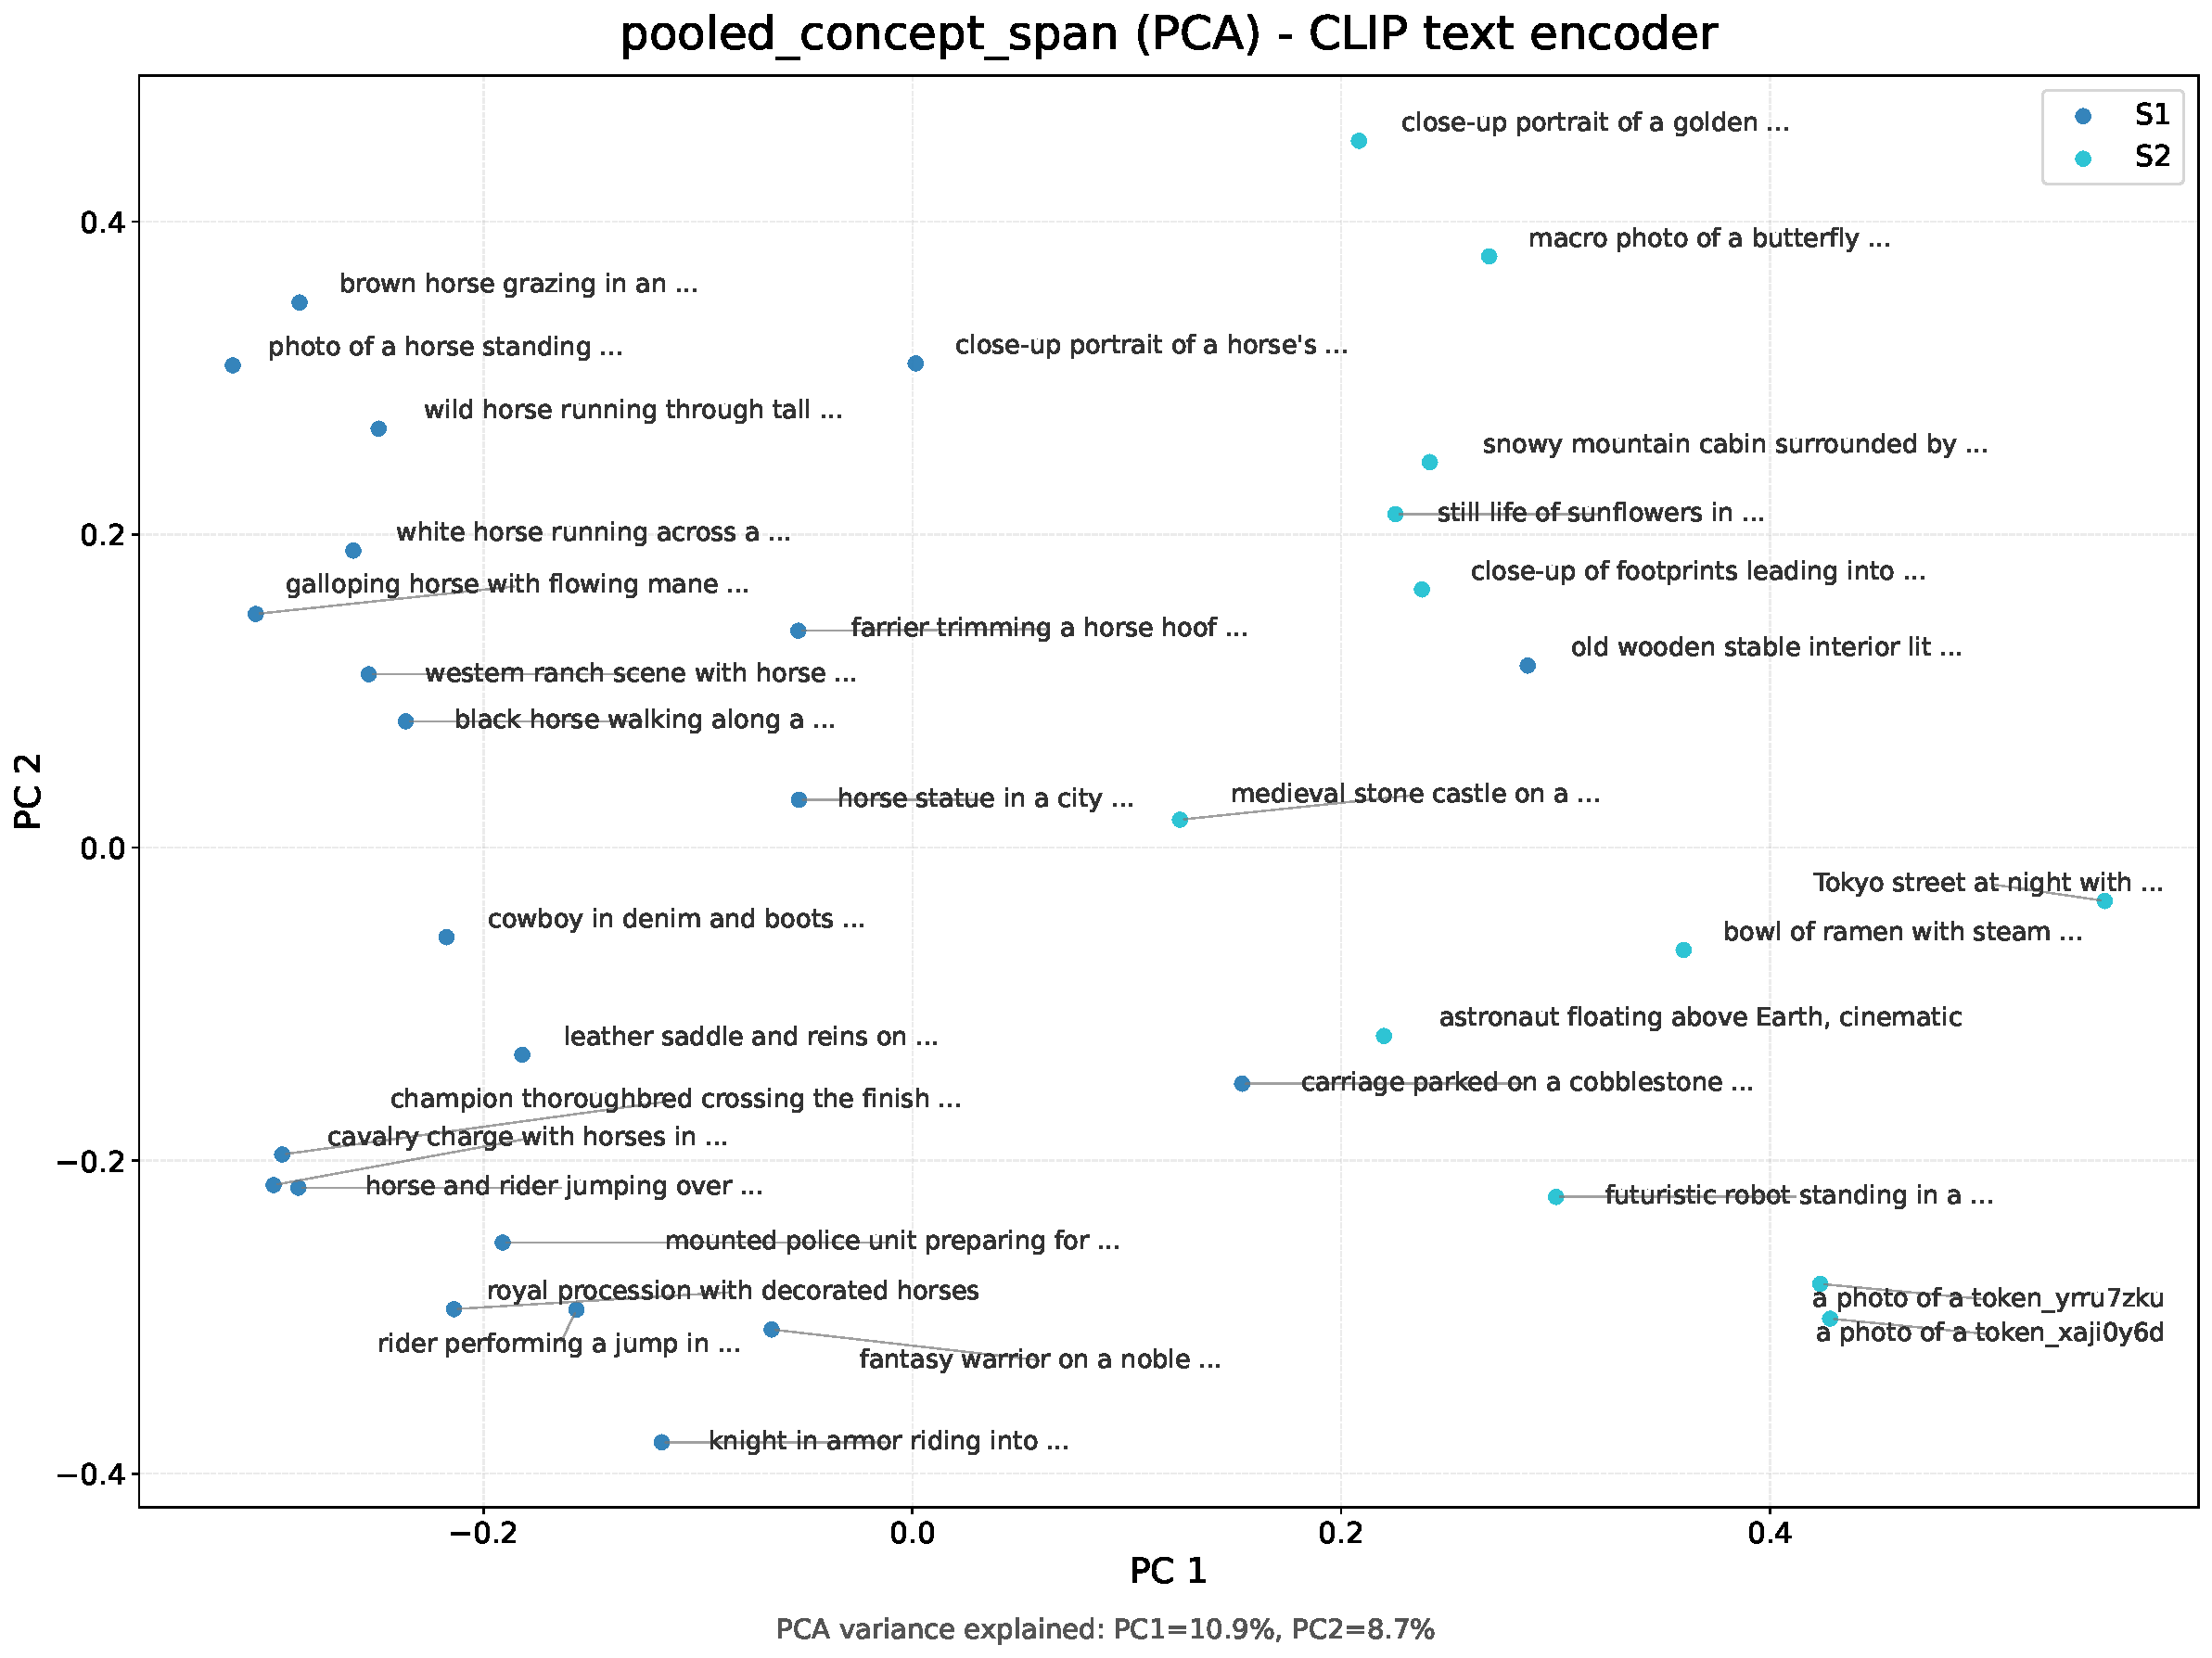
\includegraphics[width=\linewidth]{img/bag_of_words_span.pdf}
\caption{
\textbf{Context-only prompts remain close to target prompts in CLIP text-embedding space.}
PCA projection of pooled prompts used for the \texttt{horse} case study. One group explicitly contains the concept token, while the other omits it but retains correlated context words (e.g., \texttt{jockey}, \texttt{saddle}, \texttt{racetrack}). The proximity between these groups illustrates why token-level erasure can remain vulnerable to indirect contextual prompts.
}
\label{fig:bow_context_span}
\end{figure}


\paragraph{Indirect recovery prompts.}
We use the correlated context set for $c$ to construct a set of indirect prompts $\mathcal{P}_{\mathrm{ind}}(c)$. These prompts are generated under an explicit lexical exclusion constraint: they must not contain the target token or excluded lexical variants of $c$. Intuitively, $\mathcal{P}_{\mathrm{ind}}(c)$ probes whether the erased concept can still be elicited through contextual associations alone, without direct lexical mention. To improve prompt diversity while preserving control, we generate multiple prompts from different subsets of the correlated context words and retain only prompts that satisfy the exclusion rule.

\paragraph{Semantic neighbors and control concepts.}
The semantic neighborhood $\mathcal{N}(c)$ is determined by the $\delta$-threshold procedure described in~\cref{app:kappa_estimation}: 
concepts whose centroid cosine distance to $c$ falls below the 25th percentile of within-pool pairwise centroid distances. This produces concept-specific neighborhoods of two to seven discovered neighbors per target (\cref{tab:kappa}).
The control set $\mathcal{C}(c) = \{\texttt{jellyfish}, \texttt{melon}, \texttt{police car}\}$ (\texttt{cactus} substituted for \texttt{melon} for \texttt{cat} and \texttt{bear}) consists of concepts with centroid distances well above the $\delta$-threshold for every target, verified to contribute zero to $\hat\kappa$ across all five targets. For each neighbor $c' \in \mathcal{N}(c)$ and control $\tilde c \in \mathcal{C}(c)$, we generate prompts that explicitly mention the concept while excluding lexical forms of the target $c$. Per-target prompt files are released in the supplementary material.

\paragraph{Classifier-based scoring.}
All images are classified using a CLIP-based classifier over a fixed vocabulary of 60 concept labels (\cref{app:vocab}). For each image, the classifier returns the top-1 label among the vocabulary. All metrics defined below are computed from these top-1 assignments.
% For each prompt set, we generate images from the base model $\mathcal{D}_\theta$ and each unlearned model $\mathcal{D}_{\hat{\theta}}$, and evaluate the outputs using a pretrained concept classifier. For indirect prompts, we measure the fraction of generated images classified as the erased concept $c$, yielding an estimate of indirect recovery. For neighbor prompts, we measure classifier accuracy on the intended neighbor concept $c'$, which captures neighbor preservation after unlearning. For control prompts, we analogously measure accuracy on the intended non-neighbor control concept. Together, these scores allow us to distinguish target-specific collateral damage on semantic neighbors from broader degradation on unrelated concepts.

\subsection{Evaluation Metrics}
\label{app:metric_defs}
Each metric is defined with respect to a base model 
$\mathcal{D}_\theta$ and an unlearned model 
$\mathcal{D}_{\hat\theta}$. We write $\mathrm{Acc}(\mathcal{D}, c, \mathcal{P})$ for the fraction of images generated by model $\mathcal{D}$ from prompts in set $\mathcal{P}$ that are classified as concept $c$ by the CLIP evaluator.

\paragraph{Erasure metrics (measuring $\varepsilon$).}
These metrics measure how effectively the target concept $c$ is suppressed in the unlearned model.
\begin{itemize}
    \item \emph{Unlearning Accuracy (UA)}: The fraction of images generated from direct prompts $\mathcal{P}_{\mathrm{dir}}(c)$ by $\mathcal{D}_{\hat\theta}$ that 
    are \emph{not} classified as $c$. 
    \begin{equation}
    \label{eq:ua}
    \mathrm{UA}(c) = 1 - \mathrm{Acc}(\mathcal{D}_{\hat\theta}, c, \mathcal{P}_{\mathrm{dir}}(c)).
    \end{equation}
    Higher UA indicates more complete erasure under explicit lexical prompts.
    \item \emph{Indirect Recovery Rate (IRR)}: The fraction of images generated from indirect recovery prompts $\mathcal{P}_{\mathrm{ind}}(c)$ by 
    $\mathcal{D}_{\hat\theta}$ that \emph{are} classified as $c$: 
    \begin{equation}
    \label{eq:irr}
    \mathrm{IRR}(c) = \mathrm{Acc}(\mathcal{D}_{\hat\theta}, c, \mathcal{P}_{\mathrm{ind}}(c)).
    \end{equation}
    Higher IRR indicates greater vulnerability to concept recovery through correlated contextual cues. In contrast to UA, IRR measures the $\varepsilon$-robust erasure property formalized in~\cref{def:robust}.
\end{itemize}

\paragraph{Retention metrics (measuring $\gamma$).}
We measure retention at three levels of granularity:
\begin{itemize}
    \item \emph{In-domain Retain Accuracy (IRA)}: The fraction of images generated from indirect prompts by $\mathcal{D}_{\hat\theta}$ that are classified as a non-target, non-neighbor, non-control concept in the vocabulary. This captures the tendency of an unlearned model to substitute unrelated concepts when indirectly prompted for the erased target.
    %\ali{are we using this metric only for the UnlearnCanvas dataset? if not, this part is confusing and not needed.
    \item \emph{Neighbor Preservation (NP)}: our primary tradeoff metric. For a target concept $c$ with semantic neighborhood $\mathcal{N}(c)$, we define
    \begin{equation}
    \label{eq:neighbor_pres}
    \mathrm{NP}(c) = \frac{1}{|\mathcal{N}(c)|} \sum_{c' \in \mathcal{N}(c)} \frac{\mathrm{Acc}(\mathcal{D}_{\hat\theta}, c', \mathcal{P}_{\mathrm{dir}}(c'))}
    {\mathrm{Acc}(\mathcal{D}_\theta, c', \mathcal{P}_{\mathrm{dir}}(c'))}.
    \end{equation}
    An NP score of $1.0$ indicates perfect preservation of neighbors after unlearning; lower values indicate proportional collateral damage. The ratio form normalizes out the base-model recognition accuracy, which differs across concepts (and which is generally below 1.0 under a 60-class vocabulary).
    % where $\mathrm{Acc}(\mathcal{D}, c')$ denotes classifier accuracy on prompts for concept $c'$ under model $M$. An NP score of 1.0 indicates perfect preservation of nearby concepts, while lower values indicate stronger collateral damage. Unlike IRA, which averages over all non-target concepts, NP focuses specifically on semantically nearby concepts that are most likely to overlap with the erased target. \textbf{Relation to $\gamma$.} NP is an operational, classifier-based proxy for the activation-level neighbor preservation error $\gamma$ in Definition~\ref{def:neighbor}. By Assumption~\ref{asm:lip}, a small activation displacement $\|\Phi_{\hat\theta}(p) - \Phi_\theta(p)\|_2$ induces a small change in concept generation probability and hence a small drop in classifier accuracy; conversely, a method that preserves $\mathrm{NP} \approx 1$ must have kept activations close in $\mathcal{H}$. NP and $1-\gamma$ therefore track the same underlying quantity up to the Lipschitz constant $L$ and classifier noise, which is what makes it the right axis against which to plot Theorem~\ref{thm:tradeoff}'s predicted Pareto frontier.
    \item \emph{Control preservation (CP)}: To distinguish neighbor-specific collateral damage from broader degradation, we additionally evaluate performance on a non-neighbor control set $\mathcal{C}(c)$. We define
    \begin{equation}
    \label{eq:cp}
    \mathrm{CP}(c) = \frac{1}{|\mathcal{C}(c)|} \sum_{\tilde c \in \mathcal{C}(c)} 
    \frac{\mathrm{Acc}(\mathcal{D}_{\hat\theta}, \tilde c, \mathcal{P}_{\mathrm{dir}}(\tilde c))}
     {\mathrm{Acc}(\mathcal{D}_\theta, \tilde c, \mathcal{P}_{\mathrm{dir}}(\tilde c))}.
    \end{equation}
    Comparing NP and CP isolates neighbor-specific collateral damage from broader degradation: a method with $\mathrm{NP} \ll \mathrm{CP}$ is damaging concepts selectively in the target's neighborhood, consistent with the propagation mechanism in~\cref{thm:tradeoff}. A method with $\mathrm{NP} \approx \mathrm{CP} \ll 1$ is causing uniform degradation across the concept space.
    % where $\tilde{c}$ denotes a control concept that is semantically distant from $c$. Comparing NP and CP allows us to determine whether a method disproportionately harms nearby concepts, rather than causing uniform degradation across the concept space.
\end{itemize}


% \paragraph{Image quality.}
% We report Fr'{e}chet Inception Distance (FID)~\citep{heusel2017gans} to verify that the observed tradeoffs are not merely artifacts of overall image-quality degradation.


\paragraph{DamageGap.} A summary statistic we introduce to quantify neighbor-selective damage: $\mathrm{DamageGap}(c) = \mathrm{CP}(c) - \mathrm{NP}(c)$. A positive DamageGap indicates that neighbors are damaged more than controls, consistent with the tradeoff predicted by~\cref{thm:tradeoff}. A DamageGap near zero indicates uniform degradation (or uniform preservation) across both sets.

\subsection{Classification Vocabulary}
\label{app:vocab}
All CLIP-based classification uses the following 60-concept vocabulary, defined as the union of the five per-target $\kappa$-estimation pools (\cref{tab:kappa}) with duplicated controls removed. The same vocabulary is used for every metric and every target, ensuring cross-target comparability.

\begin{table}[h]
\centering
\small
\begin{tabular}{p{3cm} p{10cm}}
\toprule
Category & Concepts \\
\midrule
Targets & horse, cat, dog, bear, castle \\
Equine neighbors & pony, donkey, zebra, mustang, mare, foal, stallion, mule, bison, camel \\
Feline neighbors & kitten, tiger, lion, leopard, panther, cheetah, lynx, jaguar, cougar, bobcat \\
Canid neighbors & puppy, wolf, fox, coyote, jackal, dingo, hyena, husky, labrador, beagle \\
Ursine neighbors & grizzly, polar bear, panda, cub, koala, black bear, brown bear, teddy bear, sloth bear, sun bear \\
Architectural neighbors & fortress, castle, cathedral, palace, keep, citadel, watchtower, stronghold, fortified wall, manor \\
Controls & jellyfish, melon, cactus, police car \\
\bottomrule
\end{tabular}
\caption{The 60-concept classification vocabulary used for all CLIP-based metric evaluations in~\cref{sec:experiment}.}
\label{tab:vocab}
\end{table}
\section{Per-Concept Results}
\label{app:per_concept_tables}

This appendix provides the per-concept evaluation tables underlying the averaged results in \Cref{tab:main_results_avg}. For each of the five target concepts, we report all metrics across the seven unlearning methods. The concepts span estimated entanglement coefficients $\hat\kappa \in [0.27, 0.89]$ (\Cref{tab:kappa}), enabling the $\kappa$-scaling analysis in \Cref{subsec:kappa_scaling}.

We order tables by $\hat\kappa$ in descending order to make the predicted scaling visually apparent: collateral damage (low IRA, low NP, high DamageGap) is most pronounced for high-$\hat\kappa$ concepts and attenuates as $\hat\kappa$ decreases.

\paragraph{SAeUron coverage.} 
SAeUron's released sparse autoencoder features cover the four animal concepts (\texttt{dog}, \texttt{bear}, \texttt{horse}, \texttt{cat}) but not \texttt{castle}. We mark the corresponding row with -- in \Cref{tab:per_concept_castle} and exclude SAeUron from the averaged castle entries. Attempts to substitute SAeUron's \texttt{architectures} feature for \texttt{castle} did not yield meaningful suppression of castle generation (verified by visual inspection at the default ablation multiplier); we therefore report SAeUron only on concepts where its released features apply.

\paragraph{Reading the tables.}
All tables follow the same column structure as \Cref{tab:main_results_avg}: erasure metrics (UA, IRR), retention metrics (IRA, NP, CP), and the composite DamageGap. The \emph{Original} row reports baseline rates for the unedited $\mathcal{D}_\theta$ on each concept's evaluation set; note that baseline IRA varies substantially across concepts (e.g., {0.85} for \texttt{cat} vs. {0.54} for \texttt{tower/castle}) due to differences in CLIP evaluator accuracy on each concept's in-domain object set. This per-concept baseline variation motivates our use of normalized retention ratios in~\cref{subsec:kappa_scaling}.

% ============================================================
% Per-concept tables, ordered by descending kappa
% ============================================================

\subsection{Dog}
\label{app:per_concept_dog}

\begin{table}[h]
\centering
\small
\setlength{\tabcolsep}{5pt}
\begin{tabular}{llcccccc}
\toprule
& & \multicolumn{2}{c}{\textbf{Erasure}} & \multicolumn{3}{c}{\textbf{Retention}} & \\
\cmidrule(lr){3-4} \cmidrule(lr){5-7}
\textbf{Method} & \textbf{Type} & UA$\uparrow$ & IRR$\downarrow$ & IRA$\uparrow$ & NP$\uparrow$ & CP$\uparrow$ & DamageGap$\downarrow$ \\
\midrule
Original    & --          & 0     & 27.0  & 78.92 & 100   & 100   & --    \\
\midrule
ESD         & FT          & 75.0  & 17.5  & 74.15 & 93.51 & 96.0  & 2.48  \\
SalUn       & FT          & 90.0  & 8.0   & 50.92 & 58.01 & 76.0  & 17.98 \\
EDiff       & FT          & 62.0  & 23.5  & 66.61 & 80.29 & 92.99 & 12.70 \\
\midrule
AdvUnlearn  & Robust FT   & 96.0  & 20.0  & 74.30 & 63.05 & 99.0  & 35.94 \\
STEREO      & Robust FT   & 100.0 & 1.0   & 4.76  & 1.81  & 64.0  & 62.18 \\
\midrule
SEOT        & Inf.        & 68.0  & 30.0  & 79.07 & 84.20 & 99.0  & 14.80 \\
SAeUron     & Inf.        & 78.0  & 18.5  & 8.76  & 4.27  & 73.0  & 68.72 \\
\bottomrule
\end{tabular}
\caption{\textbf{Per-concept evaluation for \texttt{dog} ($\hat\kappa = 0.89$).} Discovered neighbors include \texttt{puppy}, \texttt{labrador}, \texttt{poodle}, \texttt{husky}, and \texttt{retriever} (full list in~\Cref{app:eval_pipeline}). As the highest-$\hat\kappa$ concept in our evaluation, \texttt{dog} exhibits the most severe robustness--retention tradeoff: robust fine-tuning methods (STEREO, AdvUnlearn) achieve high UA but cause substantial IRA and NP degradation.}
\label{tab:per_concept_dog}
\end{table}

\paragraph{Observations.}
\texttt{Dog} exhibits the most severe tradeoff in our evaluation, consistent with its position as the highest-$\hat\kappa$ concept. STEREO achieves complete erasure (UA = $100$) but collapses NP to $1.81$ and IRA to $4.76$ --- effectively destroying the model's ability to generate dog-related neighbors. SAeUron shows analogous catastrophic damage (NP = $4.27$, IRA = $8.76$) despite operating at inference time, suggesting that even modest displacement can wreck retention when neighbor activation regions densely overlap the target. ESD stands out as the only method achieving meaningful erasure (UA = $75$) while preserving neighbors well (NP = $93.51$, DamageGap = $2.48$), at the cost of higher residual leakage (IRR = $17.5$). The Pareto separation between ESD ($75, 93.51$) and STEREO ($100, 1.81$) is a $\approx 92$-point NP gap for a $25$-point UA gain, the steepest tradeoff observed across our concepts and a direct empirical instantiation of the $\kappa$-scaled lower bound predicted by~\Cref{thm:tradeoff}.

% ------------------------------------------------------------

\subsection{Bear}
\label{app:per_concept_bear}

\begin{table}[h]
\centering
\small
\setlength{\tabcolsep}{5pt}
\begin{tabular}{llcccccc}
\toprule
& & \multicolumn{2}{c}{\textbf{Erasure}} & \multicolumn{3}{c}{\textbf{Retention}} & \\
\cmidrule(lr){3-4} \cmidrule(lr){5-7}
\textbf{Method} & \textbf{Type} & UA$\uparrow$ & IRR$\downarrow$ & IRA$\uparrow$ & NP$\uparrow$ & CP$\uparrow$ & DamageGap$\downarrow$ \\
\midrule
Original    & --          & 0     & 85.5  & 62.75 & 100   & 100   & --    \\
\midrule
ESD         & FT          & 94.5  & 9.0   & 44.00 & 58.02 & 95.0  & 36.97 \\
SalUn       & FT          & 99.5  & 5.5   & 51.51 & 53.89 & 89.0  & 35.10 \\
EDiff       & FT          & 96.0  & 6.0   & 38.61 & 56.75 & 94.0  & 37.24 \\
\midrule
AdvUnlearn  & Robust FT   & 99.0  & 1.0   & 42.46 & 67.37 & 100   & 32.62 \\
STEREO      & Robust FT   & 99.5  & 2.0   & 15.88 & 13.75 & 77.0  & 63.25 \\
\midrule
SEOT        & Inf.        & 94.0  & 13.5  & 50.84 & 64.14 & 96.48 & 32.34 \\
SAeUron     & Inf.        & 85.5  & 15.0  & 22.37 & 63.50 & 93.8  & 30.30 \\
\bottomrule
\end{tabular}
\caption{\textbf{Per-concept evaluation for \texttt{bear} ($\hat\kappa = 0.82$).} Discovered neighbors include \texttt{grizzly}, \texttt{panda}, \texttt{polar bear}, \texttt{koala}, and \texttt{cub} (full list in~\Cref{app:eval_pipeline}).}
\label{tab:per_concept_bear}
\end{table}

\paragraph{Observations.}
\texttt{Bear} sits in the high-$\hat\kappa$ regime alongside horse and dog, and exhibits the predicted Pareto structure. STEREO again occupies the high-erasure / low-retention extreme (UA = $99.5$, NP = $13.75$, DamageGap = $63.25$), while AdvUnlearn achieves comparable erasure (UA = $99$) with substantially better neighbor preservation (NP = $67.37$). The clustering pattern is unusually compressed on bear: standard fine-tuning methods (ESD, SalUn, EDiff) and the inference-time methods cluster tightly between NP = $53.89$--$67.37$, with SEOT and AdvUnlearn essentially tied at NP $\approx 64$--$67$. Notably, no method on bear matches the (high UA, high NP) operating point achieved on lower-$\hat\kappa$ concepts: even ESD, the best performer on \texttt{dog} and \texttt{castle}, reaches only NP = $58.02$ here. This compression of the achievable retention region is a direct manifestation of the $\hat\kappa$-scaled Pareto frontier predicted by~\Cref{thm:tradeoff}.
\subsection{Horse}
\label{app:per_concept_horse}

\begin{table}[h]
\centering
\small
\setlength{\tabcolsep}{5pt}
\begin{tabular}{llcccccc}
\toprule
& & \multicolumn{2}{c}{\textbf{Erasure}} & \multicolumn{3}{c}{\textbf{Retention}} & \\
\cmidrule(lr){3-4} \cmidrule(lr){5-7}
\textbf{Method} & \textbf{Type} & UA$\uparrow$ & IRR$\downarrow$ & IRA$\uparrow$ & NP$\uparrow$ & CP$\uparrow$ & DamageGap$\downarrow$ \\
\midrule
Original    & --          & 0     & 75.5  & 71.23 & 100   & 100   & --    \\
\midrule
ESD         & FT          & 80.0  & 33.5  & 62.92 & 81.12 & 97.0  & 15.87 \\
SalUn       & FT          & 95.0  & 28.5  & 40.92 & 39.42 & 91.99 & 52.57 \\
EDiff       & FT          & 81.0  & 31.0  & 63.84 & 76.48 & 94.0  & 17.51 \\
\midrule
AdvUnlearn  & Robust FT   & 97.5  & 23.0  & 65.38 & 71.42 & 100   & 28.57 \\
STEREO      & Robust FT   & 100.0 & 7.5   & 20.74 & 14.71 & 27.0  & 12.28 \\
\midrule
SEOT        & Inf.        & 81.5  & 38.5  & 69.69 & 97.06 & 99.0  & 1.93  \\
SAeUron     & Inf.        & 78.0  & 39.5  & 76.92 & 82.48 & 94.0  & 11.51 \\
\bottomrule
\end{tabular}
\caption{\textbf{Per-concept evaluation for \texttt{horse} ($\hat\kappa = 0.81$).} Discovered neighbors include \texttt{pony}, \texttt{mare}, \texttt{donkey}, \texttt{zebra}, and \texttt{deer} (full list in~\Cref{app:eval_pipeline}).}
\label{tab:per_concept_horse}
\end{table}

\paragraph{Observations.}
\texttt{Horse} is the running example used throughout \Cref{sec:experiment} and exhibits the canonical Pareto structure across method families. STEREO occupies the high-erasure / catastrophic-retention extreme (UA = $100$, NP = $14.71$, IRA = $20.74$); SEOT and SAeUron occupy the high-retention / weaker-erasure region (NP $\geq 82$ but IRR $\geq 38.5$); standard fine-tuning methods sit in between, with ESD reaching a clean $(80, 81.12)$ operating point at DamageGap = $15.87$. SalUn is an outlier among standard FT methods, achieving high UA = $95$ with NP = $39.42$, far below ESD and EDiff at comparable erasure --- consistent with SalUn's gradient-saliency masking displacing more activation than necessary for erasure. A second notable observation is STEREO's collapsed CP = $27$, far below STEREO's CP on the other four concepts (range $64$--$96$): in this high-$\hat\kappa$ regime, STEREO's adversarial subspace appears to spill beyond the intended object subspace into stylistically-correlated features, manifesting the broad subspace suppression discussed in~\Cref{rem:stereo}.
\subsection{Cat}
\label{app:per_concept_cat}

\begin{table}[h]
\centering
\small
\setlength{\tabcolsep}{5pt}
\begin{tabular}{llcccccc}
\toprule
& & \multicolumn{2}{c}{\textbf{Erasure}} & \multicolumn{3}{c}{\textbf{Retention}} & \\
\cmidrule(lr){3-4} \cmidrule(lr){5-7}
\textbf{Method} & \textbf{Type} & UA$\uparrow$ & IRR$\downarrow$ & IRA$\uparrow$ & NP$\uparrow$ & CP$\uparrow$ & DamageGap$\downarrow$ \\
\midrule
Original    & --          & 0     & 96.0  & 85.50 & 100   & 100   & --    \\
\midrule
ESD         & FT          & 66.0  & 38.0  & 66.92 & 87.35 & 98.0  & 0.80  \\
SalUn       & FT          & 87.0  & 21.0  & 34.53 & 73.04 & 100   & 26.95 \\
EDiff       & FT          & 76.0  & 24.0  & 62.30 & 65.99 & 100   & 34.00 \\
\midrule
AdvUnlearn  & Robust FT   & 100.0 & 0.0   & 50.76 & 72.40 & 98.0  & 25.60 \\
STEREO      & Robust FT   & 93.0  & 7.0   & 27.68 & 27.60 & 90.0  & 62.40 \\
\midrule
SEOT        & Inf.        & 71.66 & 34.0  & 42.15 & 81.99 & 100   & 18.01 \\
SAeUron     & Inf.        & 72.0  & 37.5  & 60.25 & 85.63 & 96.0  & 10.37 \\
\bottomrule
\end{tabular}
\caption{\textbf{Per-concept evaluation for \texttt{cat} ($\hat\kappa = 0.77$).} Discovered neighbors include \texttt{kitten}, \texttt{lynx}, \texttt{leopard}, \texttt{tiger}, and \texttt{cheetah} (full list in~\Cref{app:eval_pipeline}). The original baseline IRA = $85.50$ reflects high CLIP-evaluator accuracy on cat's in-domain object set after correcting for kitten/cat label confusion (see~\Cref{app:evaluation_setup}).}
\label{tab:per_concept_cat}
\end{table}

\paragraph{Observations.}
\texttt{Cat} exhibits a tradeoff structure consistent with the high-$\hat\kappa$ regime, though its base IRA = $85.50$ is the highest of the five concepts, providing more retention "headroom" than other targets. STEREO again occupies the high-erasure / catastrophic-retention extreme (UA = $93$, NP = $27.60$, IRA = $27.68$), with DamageGap = $62.40$ matching its damage on horse and bear. AdvUnlearn achieves complete erasure (UA = $100$, IRR = $0$) at NP = $72.40$, demonstrating that adversarial training can preserve neighbors more effectively than STEREO at comparable erasure strength. ESD achieves a notable operating point: UA = $66$ at NP = $87.35$ with DamageGap = $0.80$, the cleanest standard-FT result on any concept in our evaluation, though at the cost of higher residual leakage (IRR = $38$). The STEREO IRA-retention ratio for cat ($27.68 / 85.50 = 0.32$) is consistent with the corresponding ratio on horse ($0.29$) and bear ($0.25$), reinforcing the $\hat\kappa$-scaling result in~\Cref{subsec:kappa_scaling}.
\subsection{Castle}
\label{app:per_concept_castle}

\begin{table}[h]
\centering
\small
\setlength{\tabcolsep}{5pt}
\begin{tabular}{llcccccc}
\toprule
& & \multicolumn{2}{c}{\textbf{Erasure}} & \multicolumn{3}{c}{\textbf{Retention}} & \\
\cmidrule(lr){3-4} \cmidrule(lr){5-7}
\textbf{Method} & \textbf{Type} & UA$\uparrow$ & IRR$\downarrow$ & IRA$\uparrow$ & NP$\uparrow$ & CP$\uparrow$ & DamageGap$\downarrow$ \\
\midrule
Original    & --          & 0     & 9.5   & 53.84 & 100   & 100   & --    \\
\midrule
ESD         & FT          & 88.0  & 6.5   & 48.15 & 83.03 & 99.0  & 15.98 \\
SalUn       & FT          & 97.0  & 1.0   & 54.76 & 67.58 & 94.0  & 26.41 \\
EDiff       & FT          & 82.0  & 2.5   & 46.46 & 87.35 & 99.0  & 18.69 \\
\midrule
AdvUnlearn  & Robust FT   & 100.0 & 1.0   & 44.00 & 83.10 & 100   & 16.89 \\
STEREO      & Robust FT   & 100.0 & 0.0   & 29.38 & 31.96 & 96.0  & 64.03 \\
\midrule
SEOT        & Inf.        & 98.0  & 6.5   & 53.84 & 98.21 & 99.0  & 0.79  \\
SAeUron     & Inf.        & --    & --    & --    & --    & --    & --    \\
\bottomrule
\end{tabular}
\caption{\textbf{Per-concept evaluation for \texttt{castle} ($\hat\kappa = 0.27$).} Discovered neighbors include \texttt{fortress}, \texttt{palace}, \texttt{citadel}, \texttt{keep}, and \texttt{manor} (full list in~\Cref{app:eval_pipeline}). SAeUron's released sparse autoencoder features do not cover \texttt{castle}; we attempted to substitute its \texttt{architectures} feature, but the resulting ablation did not yield meaningful suppression of castle generation.}
\label{tab:per_concept_castle}
\end{table}

\paragraph{Observations.}
\texttt{Castle} is the lowest-$\hat\kappa$ concept in our evaluation and demonstrates qualitatively different tradeoff behavior from the high-$\hat\kappa$ animal concepts. Several methods achieve strong erasure with minimal retention damage: ESD reaches UA = $88$ at NP = $83.03$ (DamageGap = $15.98$), AdvUnlearn achieves complete erasure (UA = $100$) at NP = $83.10$ (DamageGap = $16.89$), and SEOT reaches UA = $98$ at NP = $98.21$ (DamageGap = $0.79$, the lowest of any (method, concept) pair in our evaluation). This is qualitatively distinct from the high-$\hat\kappa$ concepts, where no method achieves both UA $\geq 90$ and NP $\geq 80$. STEREO is the notable exception: despite the low predicted $\kappa$-floor, STEREO incurs NP = $31.96$ and DamageGap = $64.03$, comparable to its damage on the high-$\hat\kappa$ animal concepts. This is the empirical illustration of \Cref{thm:tradeoff} as a \emph{lower bound} rather than a ceiling: STEREO's REO objective broadly suppresses the spanned adversarial subspace regardless of whether neighbors actually occupy the displaced region (\Cref{rem:stereo}), producing damage well above the $\kappa$-predicted floor that other methods successfully hug. The separation between STEREO and the alternatives on \texttt{castle} suggests room for $\kappa$-aware unlearning methods that achieve robust erasure without STEREO's $\kappa$-blind over-suppression.
\section{Direct Validation: Activation Displacement Scales with $\hat\kappa$}
\label{app:displacement_kappa}
\Cref{thm:tradeoff} predicts that activation displacement at neighbor prompts scales linearly with $\kappa$ for a method achieving $\varepsilon$-robust erasure. The Neighbor Preservation (NP) measure used in~\Cref{sec:experiment} is a probability-units proxy for this displacement, related through~\cref{asm:lip}. To test~\Cref{thm:tradeoff}'s prediction in the units the theorem is stated in, we measure activation displacement directly:
\[
\Delta_{\text{neighbor}}(c_u) \;=\; \mathbb{E}_{p_{c'} \sim \mathcal{N}_\delta(c_u)}\!\left[\, \big\| \Phi_{\hat\theta}(p_{c'}) - \Phi_\theta(p_{c'}) \big\|_2 \,\right]
\]
We measure $\Delta_{\text{neighbor}}$ for each fine-tuning method on each of the five target concepts using $200$ neighbor prompts per concept, with activations captured from \texttt{up\_blocks.1.attentions.1} at DDIM step $25$ of $50$. Inference-time methods are omitted: SEOT's text-embedding intervention does not propagate measurably to this layer in $L_2$ distance, and SAeUron's sparse-feature ablation produces displacement values an order of magnitude larger than fine-tuning methods, reflecting a real mechanism difference rather than direct comparability with weight-update methods.

\paragraph{Displacement scales monotonically with $\hat\kappa$.}
\Cref{tab:displacement} reports mean neighbor displacement across the five concepts and five fine-tuning methods. Four of five methods exhibit positive Spearman rank correlation between $\hat\kappa$ and displacement, with ESD showing strict monotonicity ($\rho = +1.00$) and STEREO closely tracking ($\rho = +0.90$ with a single inversion between \texttt{cat} and \texttt{horse}, whose $\hat\kappa$ values differ by only $0.04$). Across all five methods, displacement on \texttt{castle} ($\hat\kappa = 0.27$) is substantially lower than the average displacement across the four high-$\hat\kappa$ animal concepts: ratios range from $1.68\times$ (ESD) to $3.18\times$ (STEREO). The qualitative form predicted by \Cref{thm:tradeoff} --- displacement increasing with $\hat\kappa$ --- is empirically supported.

\begin{table}[h]
\centering
\small
\setlength{\tabcolsep}{6pt}
\begin{tabular}{lccccc|c}
\toprule
\textbf{Method} & \texttt{castle} & \texttt{cat} & \texttt{horse} & \texttt{bear} & \texttt{dog} & Spearman $\rho$ \\
& ($\hat\kappa{=}0.27$) & ($0.77$) & ($0.81$) & ($0.82$) & ($0.89$) & vs.\ $\hat\kappa$ \\
\midrule
ESD        & 128.4 & 194.8 & 213.6 & 221.0 & 235.4 & $+1.00$ \\
STEREO     & \phantom{0}75.9 & 234.2 & 233.4 & 240.9 & 257.0 & $+0.90$ \\
AdvUnlearn & \phantom{0}71.6 & 110.5 & 150.9 & 123.2 & 123.7 & $+0.70$ \\
EDiff      & \phantom{0}67.8 & 163.0 & 178.1 & 172.1 & 175.6 & $+0.70$ \\
SalUn      & \phantom{0}88.1 & 220.7 & 215.6 & 220.4 & 215.3 & $+0.10$ \\
\bottomrule
\end{tabular}
\caption{\textbf{Mean activation displacement at neighbor prompts.} Each cell reports $\Delta_{\text{neighbor}}$ in $L_2$ activation distance, averaged over $200$ neighbor prompts. Spearman $\rho$ is computed across the five concepts. Note that $n = 5$ concepts limits the statistical power of significance testing on individual methods; we report $\rho$ as a descriptive monotonicity measure. The consistency of positive correlations across four of five methods (range $+0.10$ to $+1.00$) provides aggregate evidence for the $\kappa$-scaling predicted by~\Cref{thm:tradeoff}.}
\label{tab:displacement}
\end{table}

\paragraph{STEREO's displacement is consistent with a single local Lipschitz constant.}
\Cref{thm:tradeoff} predicts that for a method operating exactly at the bound, the ratio $\kappa(1-\varepsilon)/(\Delta_{\text{neighbor}} + \delta)$ should equal a single Lipschitz constant $L$ across all concepts. We compute this ratio for each method using STEREO's saturated $\varepsilon \approx 0.02$ and $\delta = 0.05$. The resulting $L_{\text{tight}}$ values are reported in~\Cref{tab:l_tight}. STEREO's $L_{\text{tight}}$ varies by only $7.8\%$ across the five concepts ($L \in [0.0032, 0.0035]$); other methods exhibit spreads of $24\%$ to $57\%$. STEREO's single-$L$ consistency is precisely the quantitative prediction of \Cref{thm:tradeoff}: a method operating at the bound should exhibit a $\kappa$-and-concept-independent local Lipschitz constant. Among the five methods evaluated, only STEREO satisfies this prediction, consistent with STEREO occupying the high-$\Delta$, low-$\varepsilon$ regime where the bound is tightest.

\begin{table}[h]
\centering
\small
\setlength{\tabcolsep}{6pt}
\begin{tabular}{lcccccc}
\toprule
\textbf{Method} & \texttt{castle} & \texttt{cat} & \texttt{horse} & \texttt{bear} & \texttt{dog} & Spread \\
\midrule
\textbf{STEREO} & 0.0035 & 0.0032 & 0.0034 & 0.0033 & 0.0034 & \textbf{7.8\%} \\
EDiff           & 0.0039 & 0.0046 & 0.0045 & 0.0047 & 0.0050 & 23.6\% \\
SalUn           & 0.0030 & 0.0034 & 0.0037 & 0.0036 & 0.0040 & 29.5\% \\
ESD             & 0.0021 & 0.0039 & 0.0037 & 0.0036 & 0.0037 & 53.4\% \\
AdvUnlearn      & 0.0037 & 0.0068 & 0.0053 & 0.0065 & 0.0070 & 57.1\% \\
\bottomrule
\end{tabular}
\caption{\textbf{Per-concept $L_{\text{tight}}$ values.} $L_{\text{tight}} = \kappa(1-\varepsilon)/(\Delta_{\text{neighbor}} + \delta)$ is the Lipschitz constant value that places \Cref{thm:tradeoff}'s bound exactly at the observed displacement. If a method operates at the bound, $L_{\text{tight}}$ should be approximately constant across concepts. STEREO is the only method exhibiting this consistency ($7.8\%$ spread), supporting its operation at the bound's saturated-erasure regime.}
\label{tab:l_tight}
\end{table}

\paragraph{Local versus global Lipschitz.}
The local $L \approx 0.0034$ inferred from STEREO's displacement is much smaller than the global $\hat L = 0.174$ reported in~\Cref{fig:lipschitz}. This reflects the well-known phenomenon that probability changes saturate near classification decision boundaries: the global Lipschitz constant measured across diverse prompt-pair perturbations averages over both saturated and unsaturated regimes, while the local constant near $\mathcal{R}_{c_u}$ during erasure reflects unsaturated behavior specifically. The two values are compatible measurements of different but related quantities; principled estimation of $L$ that distinguishes these regimes is a direction for future work.
% \paragraph{Hierarchical metrics (for style experiments).}
% For style unlearning experiments, we additionally report:
% \begin{itemize}
% \item \emph{Parent Reversion Rate (PRR)}: the fraction of images generated from prompts targeting an erased child style $S_{\mathrm{child}}$ that are classified as either the parent style $S_{\mathrm{parent}}$ or a sibling style $S_{\mathrm{sibling}}$. A PRR substantially above the base rate indicates structured reversion toward nearby styles rather than random degradation.
% \end{itemize}
